\documentclass[12pt,pdfa]{toptesi}
%\documentclass[12pt,a4paper]{toptesi}
%\usepackage[english]{babel} 
%\usepackage{toptesi}
\usepackage[breaklinks=true]{hyperref}
\hypersetup{%
    pdfpagemode={UseOutlines},
    pdfstartview={FitH},
    colorlinks,
    bookmarksnumbered,
    plainpages,
    a4paper,
    citecolor=black,
    filecolor=black,
    linkcolor=black,
    urlcolor=black
  }
%\usepackage[square]{natbib}
\usepackage{cite}
\usepackage{graphicx}
\usepackage{amsmath}
\interdisplaylinepenalty=2500
\usepackage{amsfonts}
\usepackage{amssymb}
\usepackage{amsthm}
\usepackage{bm}
\usepackage{pstricks}
\usepackage[footnotesize]{caption}
\usepackage{subfigure}
\usepackage{float}
\usepackage{floatflt}
\usepackage{multirow}
\usepackage{textcomp}
\usepackage{setspace}
\usepackage{eurosym}
\usepackage{lscape}
\usepackage[chapter]{algorithm}
\usepackage{algpseudocode}
%\usepackage{lineno}
\usepackage{url}

\newenvironment{dedication}
  {\clearpage           % we want a new page
   \thispagestyle{empty}% no header and footer
   \vspace*{\stretch{1}}% some space at the top 
   \itshape             % the text is in italics
   \raggedleft          % flush to the right margin
  }
  {\par % end the paragraph
   \vspace{\stretch{3}} % space at bottom is three times that at the top
   \clearpage           % finish off the page
  }

\inputencoding{utf8}
%\linenumbers
\def\nr{\ensuremath{n_{\mathsf{R}}}}
%...
\def\CC{{C\nolinebreak[4]\hspace{-.05em}\raisebox{.4ex}{\tiny\bf ++}}}
\newcommand{\code}[1]{\texttt{#1}}

\begin{document}
\english
%==========================PAGINA DI COPERTINA=========================================================================
\thispagestyle{empty}
%==========================DEFINE TITLE PAGE===========================================================================
%\begin{titlepage}
\begin{center}
{\LARGE Universit\`a degli Studi di Torino}\\ \vspace{0.2cm}
{\large Dipartimento di Fisica Sperimentale}
\rule{150mm}{0.5mm}
\begin{figure}[h]
\centering
\resizebox{5cm}{!}{
\includegraphics{unitologo.png}}
\end{figure}
\\ \vspace{0.1cm}
{\Large \bf Scuola di Dottorato in Scienza ed Alta Tecnologia}\\ \vspace{0.1cm}
{\Large Indirizzo di Fisica ed Astrofisica}\\ \vspace{0.2cm}
{\Large XXVIII Ciclo}

\vspace{1.0cm}
\Huge{ \textbf{Fast GPU Nearest Neighbors search algorithms for the CMS experiment at LHC}}

\end{center}

\vspace{0.75cm}
\begin{flushright}                  
\begin{tabular}{rl}
\textbf{\large Candidato:}&  \textbf{\large Alessandro Degano}\\
 & \\
\textbf{\large Tutor:}&  \textbf{\large Prof.\ Stefano Argir\`o}\\
 & \\
\textbf{\large Coordinatore:}&  \textbf{\large Prof. Mauro Gallio}
\end{tabular} 
\end{flushright}

\vspace{0.3cm}
\begin{center}
{\large Anno accademico 2015-2016}\\
\end{center}


\newpage
\thispagestyle{empty}
\mbox{}
\newpage


\clearpage
\pagenumbering{roman}
\chapter*{Abstract}
\thispagestyle{empty}
The increase in instantaneous luminosity, number of interactions per bunch crossing and detector granularity will pose an interesting challenge for the event reconstruction and the High Level Trigger system in the CMS experiment at the High Luminosity LHC (HL-LHC), as the amount of information to be handled will increase by 2 orders of magnitude.\\
In order to reconstruct the Calorimetric clusters for a given event detected by CMS it is necessary to search for all the "hits" in a given volume inside the Calorimeter. In particular, the forward regions of the Electromagnetic Calorimeter (ECAL) will be substituted by an innovative tracking calorimeter, the High Granularity Calorimeter (HGCAL) equipped with $6.8\times10^6$ readout channels. Online reconstruction of the large events expected at HL-LHC require the development of novel, highly parallel reduction algorithms.\\
In this work, we present algorithms that,  levering the computational power of a Graphical Processor Unit (GPU), are able to perform a Nearest-Neighbors search with timing performances compatible with the constraints imposed by the Phase 2 conditions.\\
We will describe the process through which the sequential and parallel algorithms have been refined to achieve the best performance to cope with the given task. In particular, we will motivate the engineering decisions implemented in the highly-parallelized GPU-specific code, and report how the knowledge acquired in its development allowed to improve the benchmarks of the sequential CPU code.\\
The final performance of the Nearest Neighbors search in $3\times10^5$ points randomly generated following a uniform distribution is 850\unit{ms} for the sequential CPU algorithm (on an Intel i7-3770) and  41\unit{ms} for the GPU parallel algorithm (on a Nvidia Tesla K40c), resulting in an average speedup of $\sim$20.\\
The results on different hardware testbeds are also presented along with consideration on the power requirement.\\

\cleardoublepage

\indici

\pagenumbering{arabic}
% \addtocounter{chapter}{4}
%\setcounter{page}{0}
\chapter{Introduction}\label{ch:intro}
The Large Hadron Collider (LHC) is the world's largest and most powerful particle collider. It was built by the European Organization for Nuclear Research (CERN) between 1998 and 2008. From the early 2010 up until today it has produced several proton run yielding a great amount of data gathered by the four main experiments (CMS, ATLAS, ALICE and LHCB). The data allowed for the publication of hundreds of articles and between those one of the most important: the experimental confirmation of the Higgs Boson existence.\\ The current configuration of LHC will remain substantially unvaried until 2023 when, during the Long Shutdown 3 (LS3), several upgrades of the accelerator, will allow a significant increase of the instantaneous luminosity delivered. The upgraded version of the collider is referred to as High Luminosity Large Hadron Collider (HL-LHC).

\section{HL-LHC}
It is expected that by 2023 the quadrupoles magnet that focus the proton beans of LHC for the two biggest experiment (CMS and ATLAS) will be close to the end of their life cycle due to radiation exposure. The substitution of those quadrupoles and the addition of new upgrades to optimize the bunch overlap at the interaction region, will result in a significant increase of the delivered luminosity.
The proposed operating scenario is to have $5 \times 10^{34} \unit{cm^{-2}s^{-1}}$ of instantaneous luminosity, roughly five times more than the current one.\\
As a direct consequence of the increase in luminosity a high number of events happening during the same bunch crossing is expected, this phenomenon is often referred to as \textit{pileup}.\\
It is expected that an average of 140 pileup events \cite{tdr} per bunch crossing will take place as a result of the upgrade to LHC, up to spikes of 200 (while at the time of the writing the average is 22). All the main experiments will need to upgrade their detectors in order to solve the tracks originating from so many verteces and also in order to replace the components damaged by ten years of radiations with new ones able to sustain ten more years of even higher radiation.\\
As we developed this work within the CMS collaboration we focus here on the upgrades of that experiment only.

\section{CMS Phase-II upgrade}
\begin{figure}
\centerline{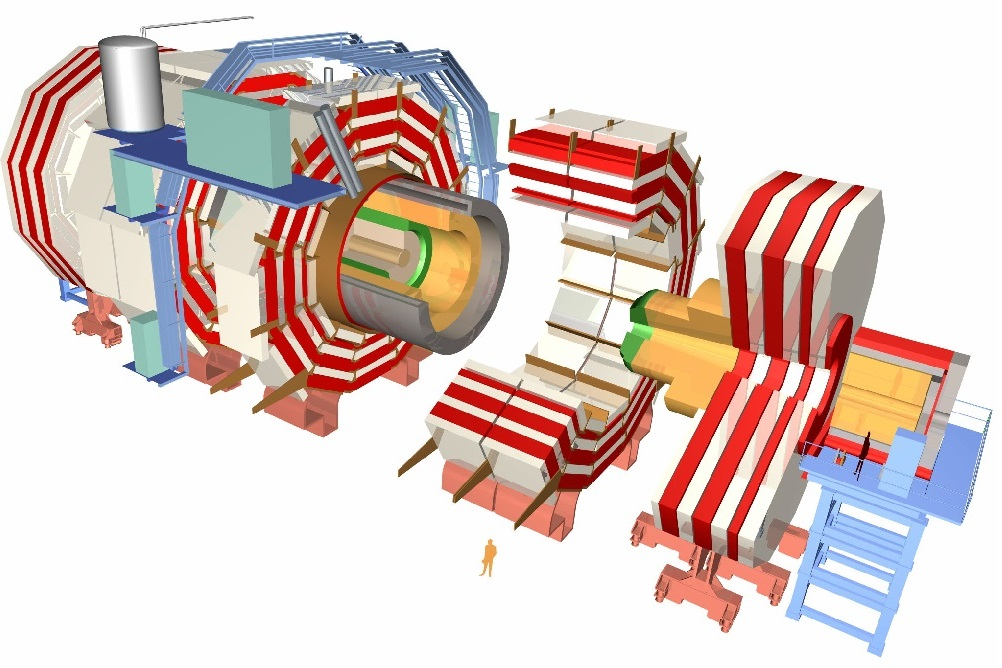
\includegraphics[width=0.8\textwidth]{intro/cms.jpg}}
\caption{An exploded view of the CMS detector in its current configuration.}
\label{cms}
\end{figure}

The Compact Muon Solenoid (CMS) is an hermetic particle detector gathering data from LHC collisions. Its general design consists of a cylinder parallel to the beam lines, called \textit{Barrel} and two discs, called \textit{EndCaps}, closing the cylinder at both ends, perpendicular to the beam lines.\\
The barrel is actually made of a series of cylindrical sub-detector each one enclosing the smaller detectors closer to the beam line. Starting from the innermost detector there is the silicon pixel tracker, followed by the silicon strips tracker. Around the tracker lies the Electromagnetic Calorimeter (ECAL), made of Lead-Tungsten crystals and followed by the Hadronic Calorimeter (HCAL) featuring brass plates interleaved by plastic scintillators. The superconducting solenoid encloses all the above and provides an inner magnetic field of 3.8 Tesla. The outermost cylinder is the one hosting the muon chambers placed between the steel return yoke that also allows the external magnetic field lines to be parallel to the beam lines and uniform. The endcaps features a similar sequence of sub-detector organized in discs of increasing radius. A detailed description of the CMS detector is given in reference \cite{cms}.\\

Following we will give a brief overview of the upgrades proposed for CMS to comply with the predicted conditions of \textit{Phase II}.

\begin{itemize}
\item \textbf{Tracker} By the time LS3 will begin the tracker, both the barrel and the endcaps, will suffer significant radiation damage -especially being the first material to be irradiated by the collisions products- and must be completely replaced. To maintain adequate track reconstructions capabilities at the conditions of HL-LHC the granularity of all the elements of the sub-detector will be increased by roughly a factor four.
\item \textbf{Calorimeter Endcaps} The forward regions of a collider detector receive the most radiation. Therefore by LS3 the Calorimeters Endcaps will also need replacement. The new calorimeter is called High Granularity Calorimiter (HGCAL) had has electromagnetic and hadronic sections with excellent segmentation. It is a sampling calorimeter where the active layers of silicon detectors are interleaved with copper and tungsten plates.
\item \textbf{Muon Endcaps} The forward muon system will receive additional chambers to maintain a good trigger acceptance. A combination of Gas Electron Multiplier and and Resistive Plate Chambers will be installed to increase the performance of the overall muon system.
\item \textbf{Low and High Level Triggers} The hardware trigger, also called Level 1, will be improved by upgrading the readout electronics in some of the sub-detectors that will be kept for Phase-II. Thus the hardware trigger rate will increase from the current 100 $\unit{kHz}$ to 750 $\unit{kHz}$ needed for the peak 200 events pileup predicted for Phase-II. Also the software trigger: called High Level Trigger (HLT), that is the one taking into account multiple sub-detectors for each event, will need to be upgraded to keep up with the increase in data rate. It is predicted that the computational power today dedicated to the HLT will need to increase up to a factor of 12.
\end{itemize}

In this work we are particularly interested by the new calorimeters endcaps, HGCAL, and the effect that the new design will have on the online reconstruction performed by the High Level Trigger. As the major difference with respect to the current sub-detector is the part dedicated to the electromagnetic detection, that is the part we mainly focus our work on.

\section{The High Granularity Calorimeter}
As mentioned above the Electromagnetic part of the HGCAL is a sampling calorimeter where layers of silicon detectors are interleaved by absorber of Tungsten-Copper.
The calorimetry usually express the thickness of the materials traversed by the electromagnetic radiations in terms of their \textit{radiation length}, denoted $X_0$, which is the mean path length required to reduce the energy of relativistic charged particles by a factor $1/\mathrm {e}$. The calorimeter is then composed of 28 layers each having an absorber and a plane of silicon detector. In details the thickness of the layers, in order from inward to outward, are as follow:
\begin{itemize}
\item 10 layers: 0.65 $X_0$
\item 10 layers: 0.88 $X_0$
\item 8 layers: 1.26 $X_0$
\end{itemize}
Resulting in a total length of 26 $X_0$.\\
The modules are shaped as two adjacent hexagons as shown in figure \ref{hgcalMod}, then they will be mounted in several copper and tungsten absorber ``petals'' which in turns will be inserted in the ``cassettes'' of the final carbon fiber structure \ref{hgcalStruct}.

\begin{figure}
\centerline{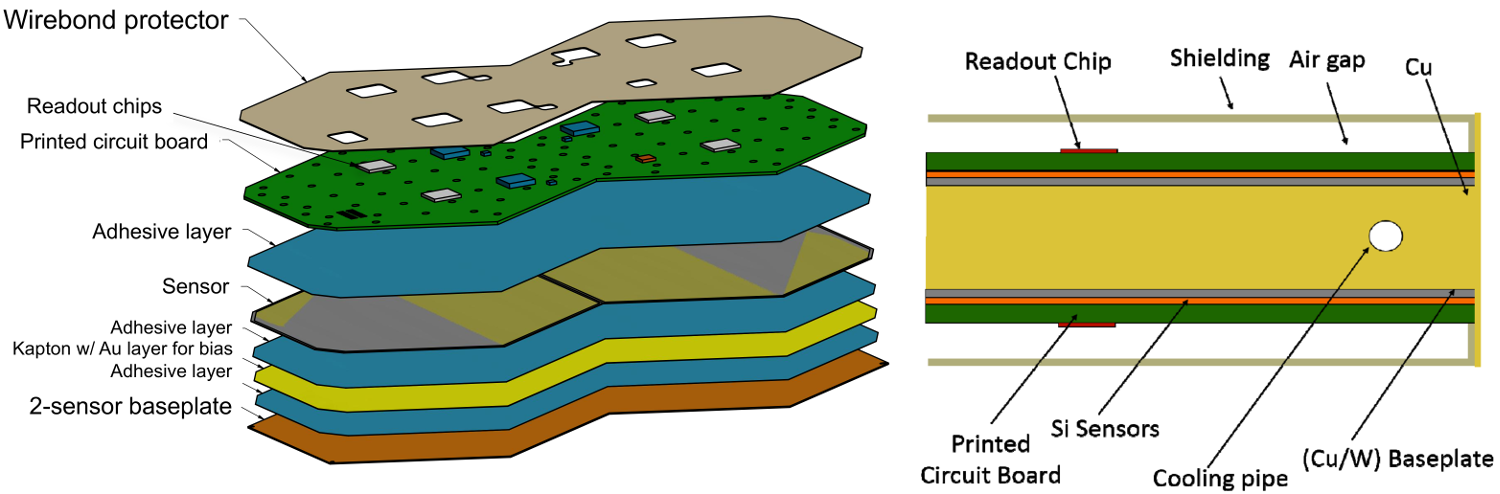
\includegraphics[width=0.8\textwidth]{intro/hgcalMod.png}}
\caption{(Left) A module of HGCAL, consisting of printed circuit board, silicon sensor and absorber. (Right) Two modules mounted on either sides of a copper tungsten absorber also used for the cooling of the system.}
\label{hgcalMod}
\end{figure}

\begin{figure}
\centerline{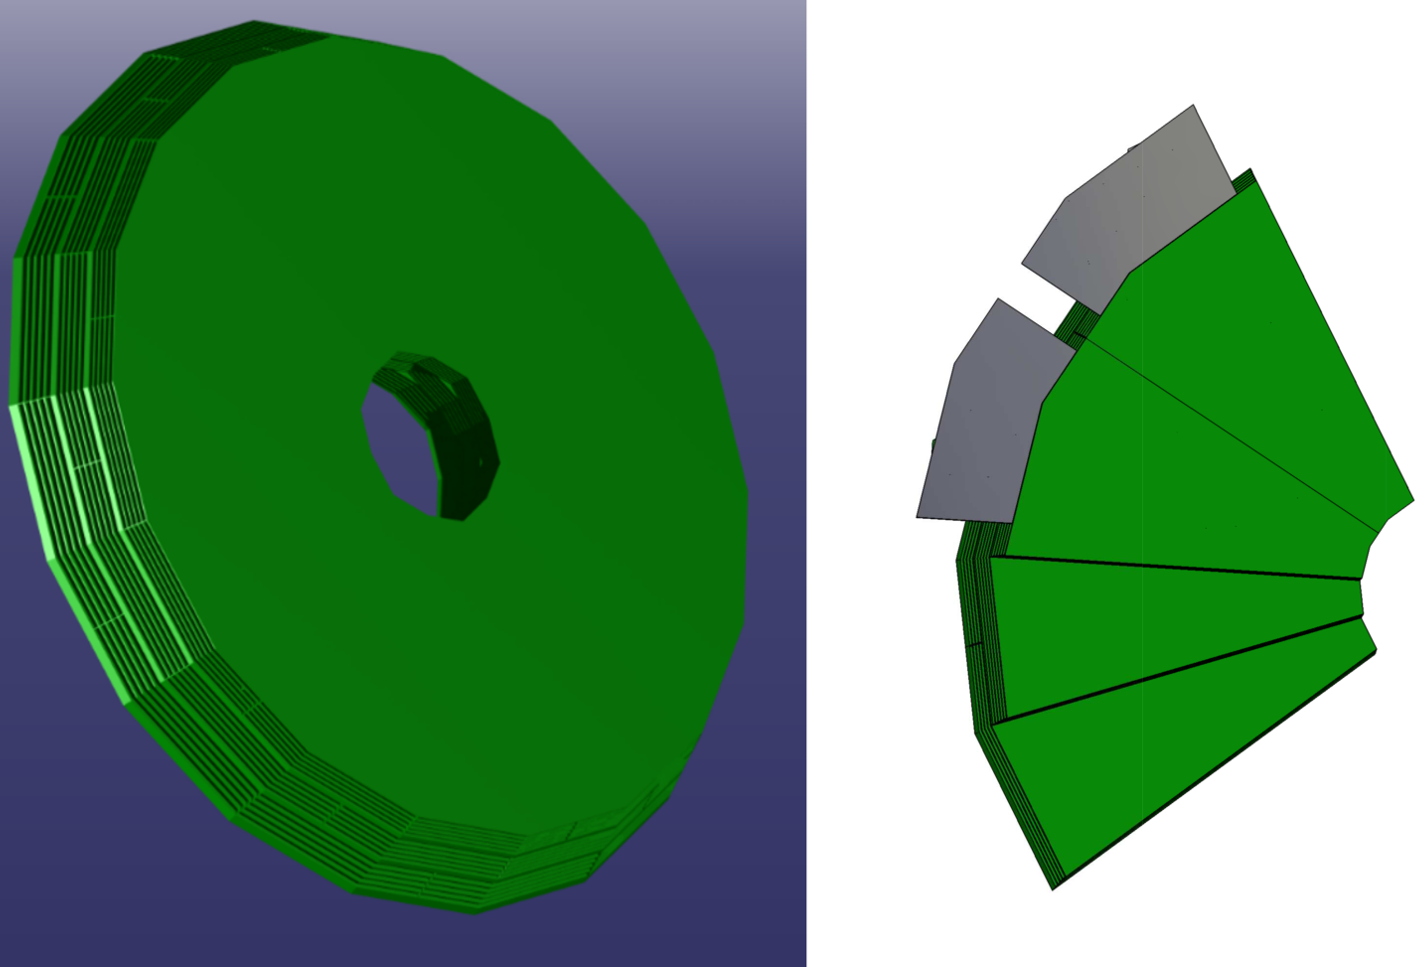
\includegraphics[width=0.8\textwidth]{intro/hgcalStruct.png}}
\caption{(Left) The final Electromagnetic HGCAL endcap carbon-fiber structure. (Right) The petals inserted into the slots of the structure.}
\label{hgcalStruct}
\end{figure}

The modules have an active area of 1.05 $\unit{cm^2}$ or 0.53 $\unit{cm^2}$ depending on their position in the endcap. Totally approximately 22000 modules will constitute the calorimeter providing a total area of active silicon of 320 $\unit{m^2}$ that will be read out by 4.3 million channels.\\


\section{Clustering overview}\label{sec:hgcal_clustering}

\section{HLT for HGCAL needs}

\section{Computation challenges}

\chapter{GPU Architecture}\label{ch:gpu}

\section{Many-cores platform and memory hierarchy}\label{sec:gpu_arch}

\section{CUDA}

\section{Testing hardware}\label{sec:benchmark}
\chapter{K-Dimensional binary search tree}\label{ch:volume_kd}
As we mentioned in Paragraph \ref{sec:hgcal_clustering} in order to form the HGCAL clusters a nearest neighbors search is required. In this chapter we describe one of the known algorithms to efficiently search for nearest neighbors in a large data set.\\
A k-d tree is a data-structure used to partition a k-dimensional space and is a special case of a binary-search tree.

\section{General description of the KD-tree}
A binary tree is a data-structure in which each element of the data-set is hierarchically connected to the other elements which also constitute the so called nodes of the tree.\\
Each node has at most two children, usually referred to as left-child and right-child. Thus from every node of a binary tree develops another sub-tree. The nodes of the tree that does not have any children are called \textit{leaves}.\\
A k-d tree subdivides a k-dimensional space in such a way that the relation between sub-spaces can be represented through a binary tree.
For all intents and purposes of this work, from here on we will consider k=3, therefore always referring to a three-dimensional Cartesian space, however all the following methods and techniques can be extended to any number of dimensions in any basis.
  
\subsection{Building a 3D tree}
The procedure of the tree construction is recursive: a starting point is chosen and it will be called the root of the tree, a plane passing through the root point and orthogonal to one of the axis defines the regions of the two sub-trees children of root, for each of those a new root is chosen between the points of the sub-tree repeating the procedure until all the sub-trees contains no points, those are the leaves of the tree.\\
In order to construct a balanced tree, where each sub-tree of a given level contains the same amount of points, there are two requirements: the first is that the subdivision must be performed cycling along the Cartesian axes, so if the first splitting is done by a plane orthogonal to $x$, the second will be done with respect to $y$, the third to $z$, the fourth again through $x$ and so on until all the leaves are created.\\
The second requirement is to choose the root of each sub-tree in such a way that both of its sons will contains the same amount of points (with the exception of one point in case of odd numbering that will conventionally be assigned to the left son). To achieve that all the points of a sub-tree are sorted according to their coordinate in the axis along which the sub-tree will be divided, the root will be the middle point defined by that with as many points preceding as many following it.\\
The relations between each node and its sons is then recorded and the procedure stops when all the elements of the set are also nodes of the tree.

\subsection{Traversing a 3D tree}
The purpose of creating a binary tree data-structure is to greatly reduce the number of comparisons required to search a given point -and/or its neighbors- in the whole set.\\
The procedure is again recursive: consider for instance the search of the nearest neighbor of an arbitrary input point among the points of the data set: using the same axes-cycling described in the building evaluate if the point is smaller or greater than the root along the axis picked. If it is smaller the search will continue on the left-child of the root, otherwise on the right-child. The second step is to compare the point to be searched with the node child of root chosen by the previous step, again comparing it along the next axis in the cycle (always maintaining the same axis-cycling order used in the construction). The procedure continues until a node without any child is reached: a leaf, which is the closest point of the set to the input point.\\
Considering the procedure described above it is clear that this type of search discards half of the points of the data set at each step. It is therefore expected that the complexity of this search is $\mathcal{O}(\log{} n)$ where simply comparing the input point to all the points in the data set would have complexity $\mathcal{O}(n)$ where $n$ is the total number of points in the data set.\\
The nearest neighbors search is just a slight variation of the above described procedure that is all the points in the data-set contained in a volume centered around an input point. The search procedure for the ``box" would be similar to the one explained for the single nearest neighbor, the only caveat being that the box can be not only ``left" or ``right" of a given node but also intersecting it. In the case of intersection both child of the node are considered for further searching. The complexity of this case has to be worse than that of a single point, in particular has been demonstrated \cite{worst-case-search} that the worse-case run-time is $\mathcal{O}(k n ^{1 - {1\over k}})$ for a k-dimensional tree of $n$ elements.

\section{Volume kd-tree}
A possible implementation of the above-described algorithm uses as tree nodes volumes in the 3D space that splits the space in which the data set points lies. Therefore the root node will be the smallest volume containing all the data set points, its children will be each half of the root, their children a quarter and so on until the leaves are created.\\
The advantage of such an implementation is that every sub-tree describes the 3D region containing all of its elements, therefore, when performing a nearest neighbors search, the search box is compared with volumes of decreasing size (the nodes of the tree) up to a point where the search box fully encloses a node: at this stage the search procedure can halt without reaching the leaves, since all the nearest neighbors are the points of the sub-tree reached, which are known because of the tree structure.\\

Following we will describe the specific implementation of the volume kd-tree we developed for this work.
\subsection{Build}
As mentioned above this implementation uses volumes as nodes of the tree which, being \textit{rectangular cuboids} in a 3D Cartesian space, can be described by only two triplets: the coordinates of the \textit{minimum} and the \textit{maximum} vertices. Where the minimum vertex is defined to be the one where each coordinate is the smallest, while the maximum the one with the greatest coordinates. This method of describing the tree nodes will benefit both the memory footprint of the tree and the process of comparing the search box position with respect to the tree nodes.\\
The building is performed similarly to what described in the generic kd-tree with the exception that for every iteration splitting in half the volume, two new volumes are created (the children).\\
For this implementation the splitting plane passes through the median point among the set contained in that sub-tree, which is found by using the \textit{tbb::parallel\_sort} method provided by Intel's Threading Building Blocks library \cite{intel_tbb} to parallelize the sorting on the CPU when a multi-core processor is available.\\
The left-child is then defined to have the same minimum vertex of its parent, while the maximum is the same of the parent except for one coordinate: the one along the axis of the splitting. That coordinate is then the same of the median point found by sorting the set. The right-child is built similarly by substituting the coordinate in the minimum vertex. The procedure is described by algorithm \ref{volume_kdtree_build}.\\

\begin{algorithm}
\caption{The build of the volume 3D-tree}
\label{volume_kdtree_build}
\begin{algorithmic}
\State BuildKDTree(totalNuberOfPoints, allPoints, 0) \Comment First call
\Procedure{BuildKDTree}{numberOfPoints, points, depth}
  \State axis $\gets$ depth $\bmod$ 3 \Comment 0 = $x$, 1 = $y$, 2 = $z$
  \State medianValue $\gets$ ceil(numberOfPoints / 2) \Comment The index of the median point
  \State \textbf{sort}(points, axis) \Comment Parallel sort of the input point along axis
  \State newCoordinate $\gets$ points[medianValue][axis]
  \State leftChild $\gets$ newCoordinate
  \State rightChild $\gets$ newCoordinate
  \State tree $\gets$ leftChild
  \State tree $\gets$ rightChild
  \If{(remainderPoints $>$ 0)}
  \State \textbf{return} \small{BuildKDTree(ceil(numberOfPoints/2), remainderPoints, depth+1)}
  \EndIf
\EndProcedure
\end{algorithmic}
\end{algorithm}

\subsection{Range search}
The search for the nearest neighbors of a given point begins by defining a region of the space to search the neighbors in.
The ``search box" is defined by the pair of coordinates describing a volume enclosing the point for which the neighbors are searched. The search is again recursive, it starts from the tree's root node. The minimum and maximum coordinates of the search box along the root's splitting axis are compared to the minimum and maximum coordinates of the children nodes along the same axis where the division took place at the construction phase. As usual only the coordinates along the axis determined by the depth of the tree are considered: if both coordinates of the search box are within those of the left-child  the search continues there, if both are within those of the right child the search proceeds there and if the search box coordinates are across both children the search proceeds on both of those nodes. In the case where a child's coordinates are within those of the search box then all the points of the child are considered as nearest neighbors and the search stops. Otherwise the search stops when a leaf is reached.\\
The whole procedure is illustrated in algorithm \ref{volume_kdtree_search}.\\
\begin{algorithm}
\caption{The build of the volume 3D-tree}
\label{volume_kdtree_search}
\begin{algorithmic}
\State SearchKDTree(searchBox, root, 0) \Comment First call
\Procedure{SearchKDTree}{searchVolume, nodeToSearch, depth}
  \If {(nodeToSearch is a leaf)}
    \State \textbf{return} node[thisPoint]
  \EndIf
  \State axis $\gets$ depth $\bmod$ 3
  \State searchBoxMin $\gets$ searchBox[minimumVertex][axis]
  \State searchBoxMax $\gets$ searchBox[maximumVertex][axis]
  \State nodeMin $\gets$ nodeToSearch[minimumVertex][axis]
  \State nodeMax $\gets$ nodeToSearch[maximumVertex][axis]
  \If{ (searchBoxMin $\leqslant$ nodeMin \&\& searchBoxMax $\geqslant$ nodeMax)} 
  \State \textbf{return} node[points] \Comment save all node's points as NN
  \Else
  	\If{ searchBoxMin $\leqslant$ nodeMin}
  	  \State \textbf{return} SearchKDTree(searchVolume, leftChild, depth + 1)
  	\EndIf
  	\If{ searchBoxMax $\geqslant$ nodeMax}
 	  \State \textbf{return} SearchKDTree(searchVolume, rightChild, depth + 1)
	\EndIf
  \EndIf
\EndProcedure
\end{algorithmic}
\end{algorithm}

\section{Validation}
We implemented the algorithm described above in \CC\ and developed the following method to validate the results of the searches performed with the volume kd-tree.\\
Using the Standard Template Library (STL) pseudo-random uniform generator defined by the \CC 11 ISO standard we place a number of points ranging from $2 \times 10^{4}$ to $3 \times 10^{5}$ in a cube of side 100 arbitrary units (a.u.). We build a volume tree with the generated points and for each of the points we perform a range search for a cube of side ranging from 1.0 a.u to 10.0 a.u. centered on the point for which we want to search the nearest neighbors and the results are recorded.\\
As comparison we perform again the nearest neighbors search through a method called \textit{naive} since it is the simplest possible way to perform such a search: for each search box every single point of the data set is checked: if it lies inside the box it is recorded. It is also clear that the naive method is very inefficient having complexity $\mathcal{O}(n^{2})$ when searching the nearest neighbors of all $n$ points. However it is a simple and reliable method to validate less intuitive algorithms and we used it extensively as a validation tool throughout this work.\\
The data set random generation is executed for different numbers of data set points and different sizes of the search boxes and both searches -naive and kd-tree- performed, the results of the two methods are then compared for each generation and only when they are always identical the kd-tree range search algorithm is declared valid.

\section{GPU porting}
The GPU architecture we described in Chapter \ref{ch:gpu} requires some adaptations of the code to best perform on this device. We list here the most relevant:
\begin{itemize}
\item The specific parts of code that runs on the GPU must be CUDA-compliant e.g. STL containers must be avoided and only some \CC\ constructs can be used.
\item Input data must be moved on the GPU device and must have the smallest possible byte size to avoid that the data transfer rate becomes a significant bottle-neck.
\item Several processes must run simultaneously as, ideally, all the GPU computational cores must be used at the same time.
\item Output data must be moved back from the GPU device to the host machine and the size of the output data has to be known.
\end{itemize}
We first attempted to perform the tree construction on the GPU device, should that performed well not only we would have exploited the GPU computation for this part of the algorithm too, but we would have had the tree saved on the GPU memory without needing to move it. Unfortunately it became soon apparent that it wasn't possible to build the tree in a way that employed all the GPU cores at the same time and the performance were worse than those obtained on the CPU.\\
The all nearest neighbors search is much simpler to parallelize in order to fill up the GPU cores: by assigning a search box to each GPU core they can all run simultaneously and independently. Therefore once the tree is built on the host machine there are two inputs that needs to be loaded onto the GPU memory: the tree itself, which can be expressed as an array of pair of vertices of $n$ elements for $n$ data set points and the search boxes which again is an array of pair of vertices of $n$ elements.\\
The search code itself is the very same that runs sequentially on the CPU, however the code generates one CUDA thread for every search box to be found, then the GPU device scheduler takes care of executing each of those threads on all the available GPU cores, reaching the concurrential execution desired.\\
The output result is a single array where the indices of the nearest neighbors are recorded. As mentioned before the size of this array must be known before the search is performed which implies the need of an assumption on the number of nearest neighbors found for each search box. In the case of the uniform random generation of $N_{total}$ points in a volume $\mathcal{V}$ we evaluate the statistical average density of nearest neighbors found in a search box of volume $\mathcal{V_s}$ and we double the average number of points per search volume to take into account the statistical variance.
\begin{center}
\begin{equation}
N\!N_{max} =  N_{total} \cdot \dfrac{\mathcal{V_s}}{\mathcal{V}} \cdot 2.0
\end{equation}
\end{center}

Thus the array size is $N_{total} \cdot N\!N_{max}$, however most of the times the number of actual NN found is lower than the maximum allowed, therefore a trailing $-1$ is used to instruct the code reading the output that there are not any more nearest neighbors for that search box.\\
The formula described above clearly cannot be applied to real-world applications where the distribution of points is not uniform, therefore other assumptions must be evaluated.\\

\section{Performance analysis}
The assessment of the performance of the GPU algorithm is done by comparison with the same code running sequentially on the CPU.\\
The two search methods runs on the exact same points, generated by a uniform random distribution, similarly to what is done for the validation. Likewise the measurements are repeated for a series of numbers of initial points, ranging from  $2 \times 10^{4}$ to $3.5 \times 10^{5}$. The volume in which the points are generated is a cube of side 100.0 a.u. while the reference search box is a cube of side 4.0 a.u.\\
The computational time spent in each search is evaluated through \textit{cudaEvent} provided by the CUDA libraries which provides a time resolution of $\sim 0.5\unit{ms}$. The tests are performed on the benchmark machine described in Paragraph \ref{sec:benchmark}.\\
Figure \ref{volume_kdtree_build} shows the time required to build the tree for the various numbers of initial points tested, Table \ref{volume_kd_tree_tab} reports some selected results of the search times, while Figure \ref{volume_kdtree_plot} shows the search timing in a logarithmic scale for all the tests performed, lastly Figure \ref{volume_kdtree_speedup} shows the speedup between the GPU-parallel and the CPU-sequential search codes.\\

\begin{figure}
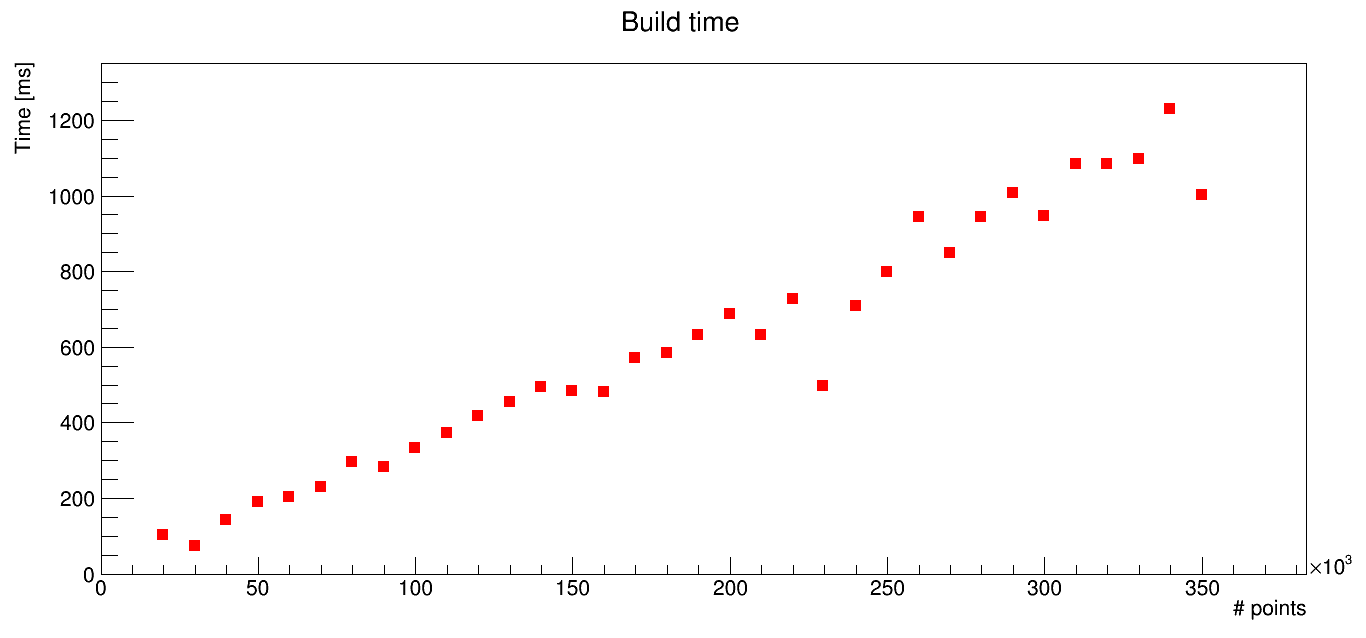
\includegraphics[width=\textwidth]{volumeKdPlot/volumeBuildTime.png}
\caption{Volume Kd-tree build timings.}
\label{volume_kdtree_plot}
\end{figure}

\begin{center}
\begin{table}[h]
\begin{tabular}{ c || r r r r r r r }
Points ($10^{3}$) & 50 & 100 & 150 & 200 & 250 & 300 & 350 \\
\hline
CPU ($\unit{ms}$) & 163.8 & 528.4 & 1186 & 2234 & 3091 & 4225 & 5501 \\
GPU ($\unit{ms}$) & 75.3 & 229.7 & 430.5 & 681.8 & 953.9 & 1281 & 1639 \\
\end{tabular}
\caption{Volume Kd-tree selected search times for CPU sequential and GPU parallel code}
\label{volume_kd_tree_tab}
\end{table}
\end{center}

\begin{figure}
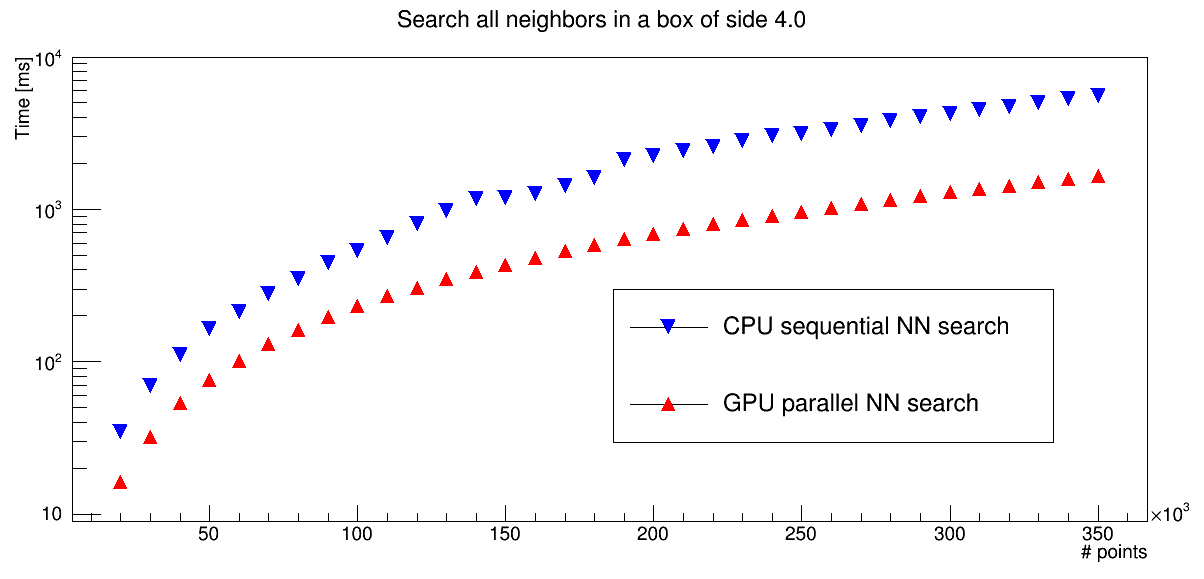
\includegraphics[width=\textwidth]{volumeKdPlot/volumeKdTree.png}
\caption{Volume Kd-tree search times for CPU sequential and GPU parallel code}
\label{volume_kdtree_plot}
\end{figure}

\begin{figure}
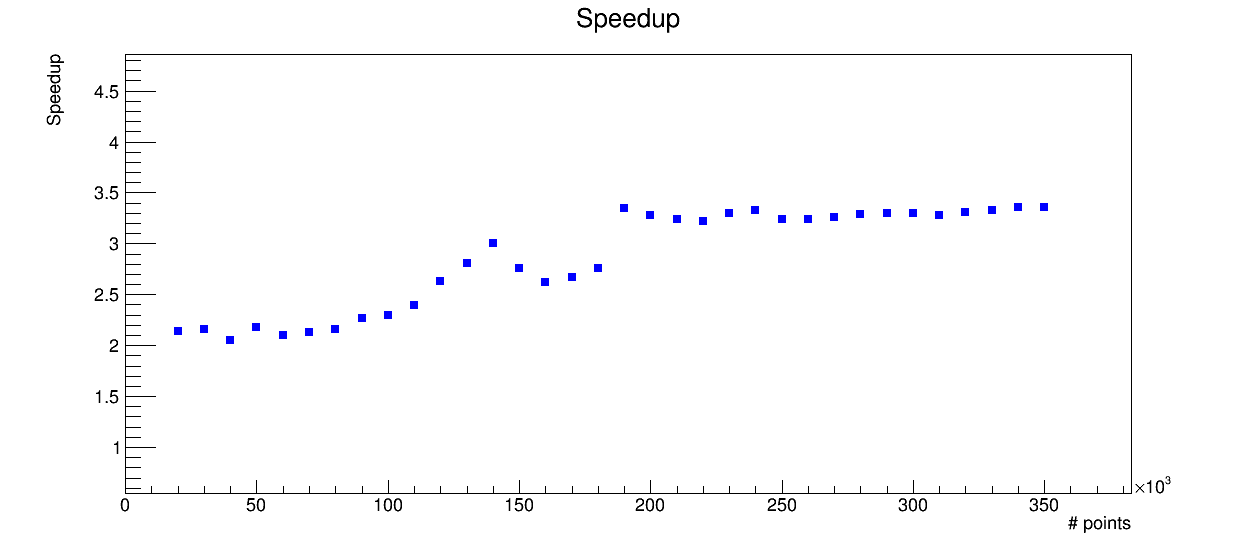
\includegraphics[width=\textwidth]{volumeKdPlot/volumeKdSpeedup.png}
\caption{Volume Kd-tree speedup between CPU sequential and GPU parallel search code}
\label{volume_kdtree_speedup}
\end{figure}
\newpage

\section{Algorithm assessment}
The build times shown in Figure \ref{volume_kdtree_build} suggests that building this kind of ``volume" tree is expensive as it can use from $\sim 25\%$ up to $\sim 100\%$ of the time employed by the search itself. Furthermore the time spent to build the tree for $3 \times 10^{4}$ points, which is $\sim 1\unit{s}$, is well past the constraints imposed by HGCAL's HLT by itself not considering the search.\\
In Figure \ref{volume_kdtree_plot} observe the relative performance of the two search methods for the lowest number of points used: in that regime the GPU parallel code is still faster than the sequential one, implying that the data transfer time needed to load the input and unload the output to/from the GPU also scales with the number of points and does not add a significative fixed time contribution to the process. This is an important feature as the algorithm must perform well in all the ranges at which it can be operated.\\
The CPU sequential timings, however, are not very encouraging requiring up to $5.5 \unit{s}$ to process the highest number of points. This result is well outside of the requirements imposed by the Phase 2 of LHC.\\
According to Figure \ref{volume_kdtree_speedup} the parallel GPU code is always faster than its sequential counterpart by a factor $\sim 2$ to $\sim 3.5$, gaining performance as the number of points to be processed increases. While this is a desired feature of the parallel code, implying that it scales well with the increase of points, the GPU code is also too slow for the requirements.\\
Further analysis of the code, performed at runtime, reveals two major issues with the algorithm developed for the range search of the volume kd-tree, regardless of its parallel or sequential implementation. The first one is caused by the way we save the tree nodes in the array: as they are not assigned to a specific place, but rather just to the last available place, at every recursion the node visited is asked for the index of its sons. The process of accessing the memory to read the indices of the node's sons is relatively expensive and it adds up quickly when repeated millions of times in all the recursions.\\
The second issue derives from a missed performance gain opportunity: despite we designed the volume kd-tree in a way that could quickly return sets of near points when the search box would contain an entire node, analysing the code running with the conditions described above, revealed that this feature is seldomly used if ever. As a matter of fact the size chosen for the volume we distribute the initial data set and the size of the search box we used for the testing are such that when the search box contains a node that is not a leaf the node is still too small compared to the total volume and contains few points, making the contribution of this feature negligible.\\
As a result of the above consideration we determine that the volume kd-tree is not the best suited data-structure for the geometry and times constraints that this work aims to tackle. The following chapter presents a different implementation of a kd-tree where the above issues has been solved.\\





\chapter{A better KD-tree implementation}\label{ch:fkdtree}
In this chapter we describe a different implementation of a KD-tree that fixes the issues of the volume KD-tree explained in Section \ref{sec:volumeKdAssessment} and implements a search much more suitable to a highly parallel computation. The implementation is again wrote in \CC\ and CUDA for the GPU relevant parts.

\section{Build of a left-balanced KD-tree}
A left-balanced binary tree is a tree in which the leaves only occupy the leftmost positions in the last level. This positioning can be applied to the leaves of a KD-tree as well by chosing to assign the leaves of the tree to the leftmost available parent.\\
In practice this can be achieved by assigning the index of each node of the tree to a pre-determined value evaluated by the node's depth in the tree and its relative position among the other nodes at the same depth.\\
The KD-tree nodes are assigned to a binary tree, therefore each node has two children in the next layer and the number of nodes $N_d$ at a given depth $d$ can be evaluated as $N_d = 2^d$ where $d = 0$ is the depth of the root. Moreover the indeces of the children of a given node of index $I_p$ can also be simply evaluated to be $I_{left} = I_p \cdot 2$ and $I_{right} = I_p \cdot 2 + 1$. Using this knowledge we assign to the nodes of the tree a pre-determined index.\\
For this implementation of KD-tree we also drop the feature used in the volume KD-tree to assign a volume to each node of the tree. In this implementation each node of the tree corresponds to one point of the data set.\\
By exploiting the predictive placement of the tree nodes we can also implement a build procedure that is iterative instead of recursive: an outer loop visits all the layers of the tree until all the leaves are created, inside another internal loop -that spans the tree horizontaly- creates one by one the children of the nodes at the current depth, assigning them the index that can be evaluated as powers of 2 as described by the above formula. The inner loops ends when all the children of the next depth are created, and the outer loop ends when each point of the data set is a node of the tree.\\
We determine the point to assign to each node by a sort performed along an axis similar to the one described in Paragraph \ref{sec:volumeKDBuild}, however in this implementation we realize that there is no reason to sort all the points in the range, what is needed, indeed, is to find the median point among them along the sorting axis, and then the points with the coordinate along the splitting axis smaller on one side and those with greater coordinates on the other side: the relative sorting in this two sets is irrelevant and can be avoided to gain some performance. The STL library provides a function that just does that: \textit{std::nth\_element} which we include in the build procedure.\\
Algorithm \ref{fkdtree_build} shows how we implemented the features described above.\\

\begin{algorithm}
\caption{The build of a left-balanced KD-tree}
\label{fkdtree_build}
\begin{algorithmic}
\Procedure{BuildKDTree}{numberOfPoints, points}
  \State pointsToEvaluate $\gets$ 0
  \For{(thisDepth $<$ maximumDepth)}
  \State axis $\gets$ thisDepth $\bmod$ 3 \Comment 0 = $x$, 1 = $y$, 2 = $z$
	  \For{ (thisIndex $<$ thisDepth$^2$)}
	  	\State medianValue $\gets$ pointsToEvaluate[thisIndex] / 2
	  	\State sortedPoints $\gets$ std::nth\_element(pointsInThisNode, medianValue)
	  	\State thisIndex $\gets$ medianValue
	  	\State tree[thisIndex] $\gets$ points[thisIndex]
	  	\State pointsToEvaluate[leftSon] $\gets$ sortedPoints[0,thisIndex)
	  	\State pointsToEvaluate[rightSon] $\gets$ sortedPoints[thisIndex, lastIndex]
	  \EndFor
  \EndFor
\EndProcedure
\end{algorithmic}
\end{algorithm}

\section{Iterative range search}
To perform a range search the algorithm takes a ``search box'' as argument for which it finds the points in the data set that are enclosed in it.\\
The search procedure, recursive by nature, is made iterative by exploiting the predictable nodes placement described by the build procedure. Particularly, starting from the root node, the algorithm checks if the node -along the splitting axis defined by the node's depth- is greater than the search box maximum vertex, smaller of the minimum vertex or if it lies in the search box. When the node is greater than the search box the search proceeds on the node's left-child, when is smaller on the right-child and when it lies within the search box both children are considered for the next step in the search and the node is recorded as a nearest neighbor and will not be checked again.\\
In order to make the above procedure iterative, avoiding the recursion, a loop is performed on all the nodes to compare the search box against. The iteration is initialized by adding to a \textit{queue} the root node index. The loop starts and compare the search box against the root, then one or both of its childrens are added to the queue while the node compared is removed from the queue. The next iteration of the cycle will compare the search box against the last element of the queue (e.g. the node(s) added on the previous step) and remove it from the queue while adding whichever children the search must proceed on. The loop repeats until the queue is empty which means that the leaves are all reached and all the nearest neighbors recorded.\\

\subsection{Fast bitwise operations}
At every step of the search the axis along which the current node has been created must be known. It can be easily deduced by knowing the depth of the tree the node is situated at, which in turns could be saved as part of the information of the node, however we decided against it to reduce to the bare minimum the memory footprint of the array of nodes. The depth of the node in the tree, indeed, can be evaluated from the node index $I$ by inverting the formula described in the previous Section, that is: $d = \lfloor log_2(I) \rfloor$ which in \CC\ can be easily implemented with the embedded C functions as: \code{d = floor(log2(I))}.\\
However we analysed the performance of the above code and found that it is relatively expensive in execution time. Therefore we replaced the code based on the C functions with a custom function leveraging the bitwise operators: \code{((unsigned int) (31 - \_\_builtin\_clz( I | 1) ))}. Starting from the inner parts the \code{I | 1} cosiders the integer representing the index of the node as a sequence of bits and does the $OR$ with the bit $1$, this ensures that the function works also in the case of $I = 0$. Then \code{\_\_builtin\_clz()} counts the number of leading zeroes in the index of the node when represented in binary form. The total number of bits representing an \code{unsigned int} in most common computer architectures is 32, therefore subtracting the number of leading zeroes of the index to 32 gives the logarithm in base two of the index. Subtracting one to that number and then performing the cast to \code{unsigned int} performs the equivalent of the \code{floor()} operation giving the expected result.\\
This seemingly harmless substitution in the code resulted in a very tangible increase in performance being up to ten times faster than the code using the C functions.\\
The implementation of the range search is showed in Algorithm \ref{fkdtree_search}.\\

\begin{algorithm}
\caption{Range search of the left-balanced KD-tree}
\label{fkdtree_search}
\begin{algorithmic}
\Procedure{SearchKDTree}{searchBox}
  \State nodesToVisit $\gets$ 0
  \While{(nodesToVisit)}
  	\State indexToCheck $\gets$ nodesToVisit[last]
  	\State thisDepth $\gets$ \textbf{FLOOR\_LOG2}(indexToCheck) \Comment as explained above
	\State axis $\gets$ thisDepth $\bmod$ 3 \Comment 0 = $x$, 1 = $y$, 2 = $z$
	\If{(searchBox[axis][min] $<=$ indexToCheck[axis] \\ \hspace{4em} \textbf{AND} searchBox[axis][max] $>=$ indexToCheck[axis])}
		\State nodesToVisit $\gets$ leftChild, rightChild
		\State nearestNeighborsResult $\gets$ indexToCheck
	\ElsIf{(searchBox[axis][max] $<=$ indexToCheck[axis])}
		\State nodesToVisit $\gets$ leftChild
	\Else
		\State nodesToVisit $\gets$ rightChild
	\EndIf		
	\State nodesToVisit $\textit{remove}$ indexToCheck
  \EndWhile
  \State \textbf{return} nearestNeighborsResult
\EndProcedure
\end{algorithmic}
\end{algorithm}

\section{Validation}
We implemented the KD-tree algorithm in \CC\ and validated it with the same technique described in Section \ref{sec:volume_kdtree_validation}, using uniformly distributed random points and comparing the search results with the \textit{naive} method.\\
As an additional validation and debug tools we implemented two recursive functions for the build and the range search respectively.
The first, through the classic recursion, verify that the nodes have the correct relative positioning among them. While the second, again recursively, verify that when searching for a single point of the data set used to build the tree, said point is indeed found in the leaf it is supposed to be.\\

\section{GPU porting}
We focus our attention on parallelizing the range search part of the algorithm and run it on a GPU. We expect to gain a significative increase in performance by running the all nearest neighbors searches in parallel assigning one search box to one CUDA thread and executing several thousand (depending on the actual GPU used) threads at the same time.\\
In order to port the algorithm described in \ref{fkdtree_search} to CUDA there are some obstacles to get around first.\\

\subsection{GPU queue}
CUDA does not support STL containers and does not provide a variable size queue (at least in version 7.5 used in this work). Therefore we made our own implementation to save the nodes indices to visit in each loop cycle.\\
The motivations to have a variable size queue are mainly two: the tree could be arbitrarily long and if the visited node index was not removed at each cycle the size of the array containing the visited nodes could become too big for the very limited registry memory each CUDA core has access to (see Section \ref{sec:gpu_arch}). The second reason is that by having a dynamic size it is always known which is the last element of the queue allowing the search to access it at every cycle and then remove it.\\
The implementation is reported in Appendix \ref{ch:appendixFKDTree}.

\subsection{CUDA streams}
The array of search boxes and the array of the nodes (the tree structure) must be both moved on the GPU memory before executing the code that performs the range search, also, the array of the index of the nearest neighbors must be copied back on the host computer once the search is completed. The time necessary to perform those copy can be a relevant fraction of the total time spent for the range search.\\
Nvidia's GPUs provides a feature that can help mitigate the time cost of copying the data to and from the device. Recent Nvidia GPUs are able to copy data to the device, from the device and execute code at the same time. Clearly to have an output to copy back on the host machine the code execution must have ran which, in turn, must have had access to the input data copied on the GPU device. Therefore to profit of the feature the whole search process must be split in what CUDA calls \textit{streams}, inside every stream the copy to the device, the execution and the copy from the device are executed sequentially, however different streams are asyncronous and indipendent. So, for instance, suppose to have two streams: the first stream begins to copy its portion of data on the device, once it is done its execution begins but, at the same time, the copy of the data on the device of the second stream begins. Likewise the stream 1 can then copy the output back to the host machine while stream 2 is still executing the code.\\
Figure \ref{cuda_streams} shows how the interleaving of the streams can ``hide'' the cost of the memory management.\\

\begin{figure}
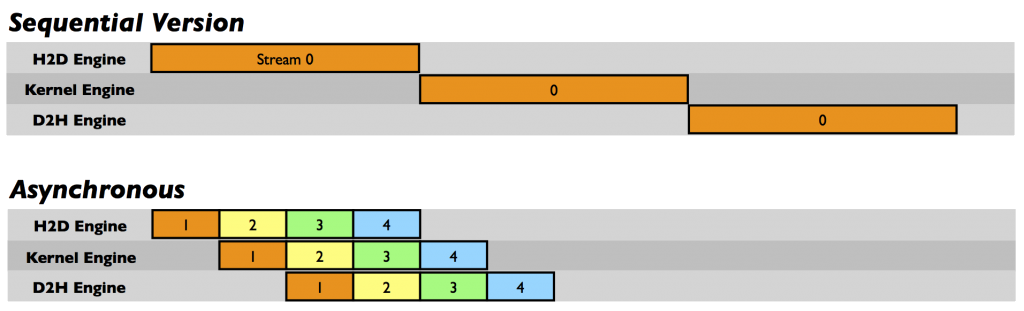
\includegraphics[width=\textwidth]{fkdtree/cuda_streams.png}
\caption{Interleaving of four asyncronous CUDA streams. H2D: host to device process, D2H: device to host, Kernel: code execution.}
\label{cuda_streams}
\end{figure}

We implemented in the search algorithm the possibility to split the all nearest neighbors search in an arbitrary number of CUDA streams to evaluate which number of streams yields the best performance.\\

\section{Performance analysis}
To evaluate the performance of this implementation we use the same method applied to the volume KD-tree used in Section \ref{sec:volumeKd_performance} with further investigation where required.\\

\subsection{Uniform random distribution}
The first set of tests are performed by building the KD-tree off a uniform random distribution of points. The data sets are produced with a number of points ranging from $2 \times 10^4$ to $5 \times 10^5$.\\
We measure the time spent building the tree, the search times differences for the GPU parallel code with different number of CUDA streams, the search times of the CPU sequential code and the speedup between the two.\\
Figure \ref{fkdtree_build_times} shows the time spent building the KD-tree for the various number of data set points.\\

\begin{figure}
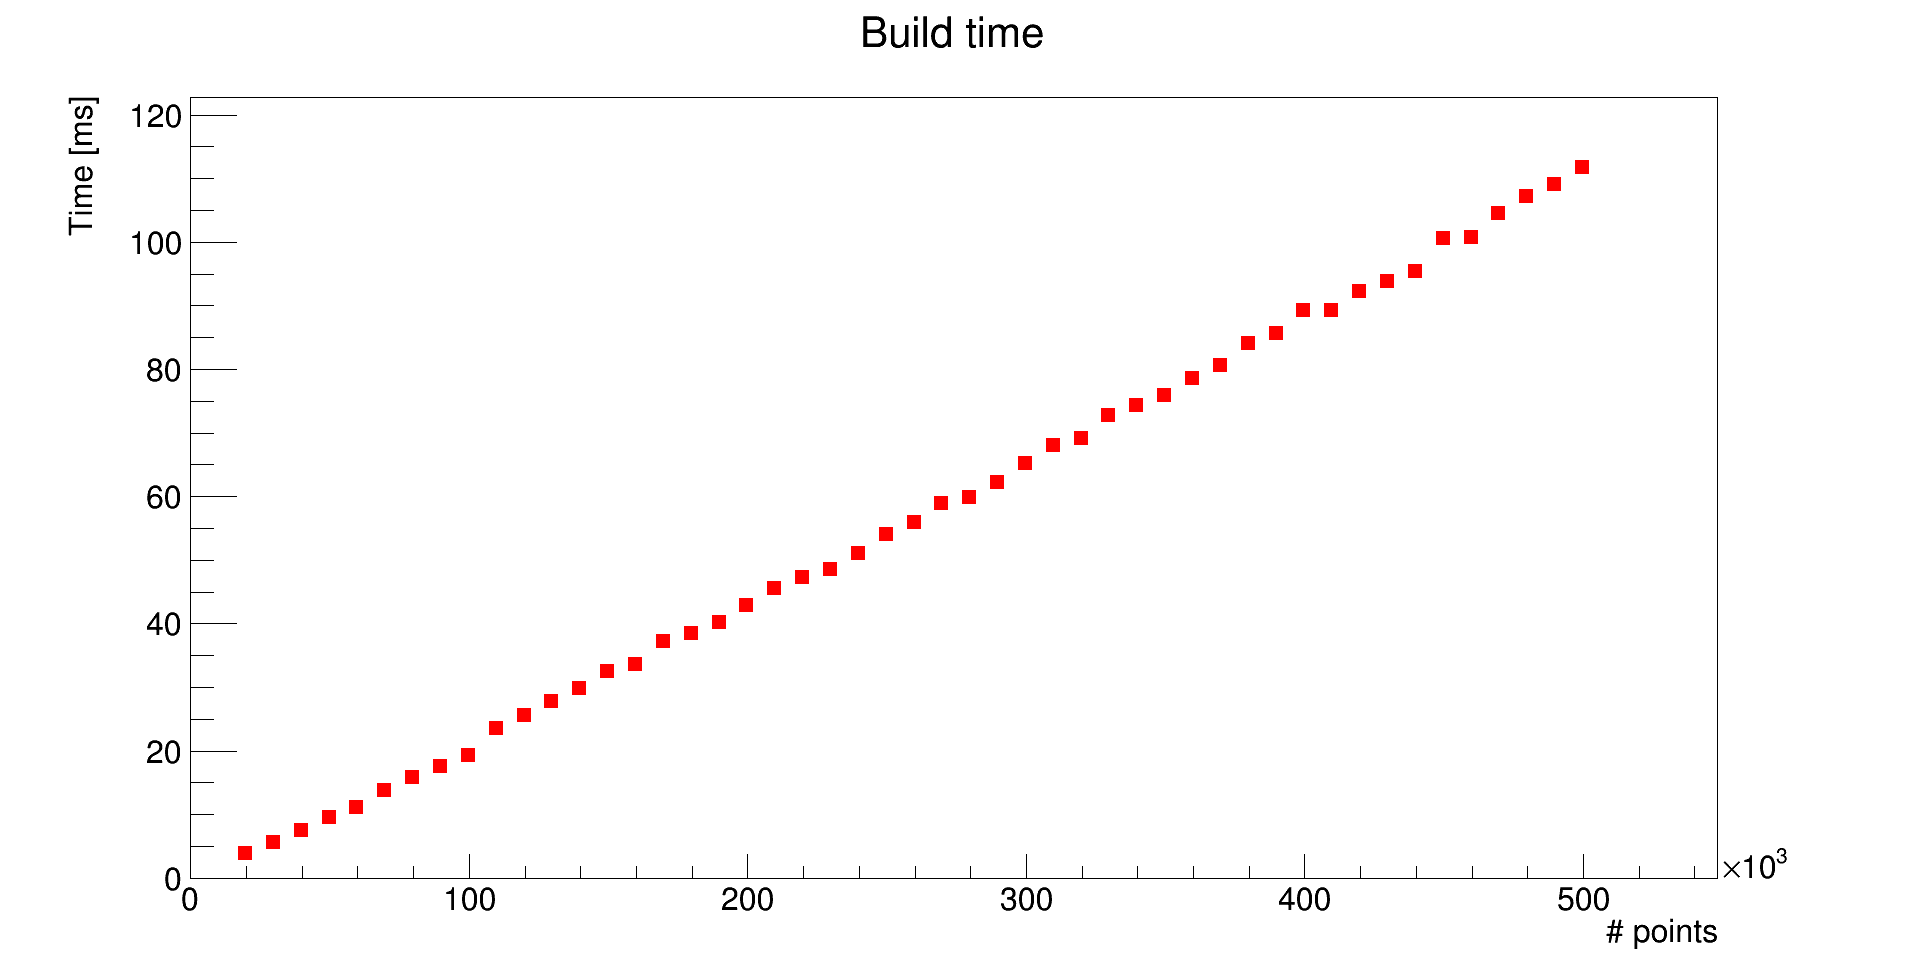
\includegraphics[width=\textwidth]{fkdtree/fkdBuildTimes.png}
\caption{Time spent by the build of the KD-tree.}
\label{fkdtree_build_times}
\end{figure}

Figure \ref{fkdtree_streams} shows the relative performance gain of the search performed with 2 to 16 CUDA streams with respect to the single stream for a number of generated points between $6 \times 10^4$ to $5 \times 10^5$.\\
\begin{figure}
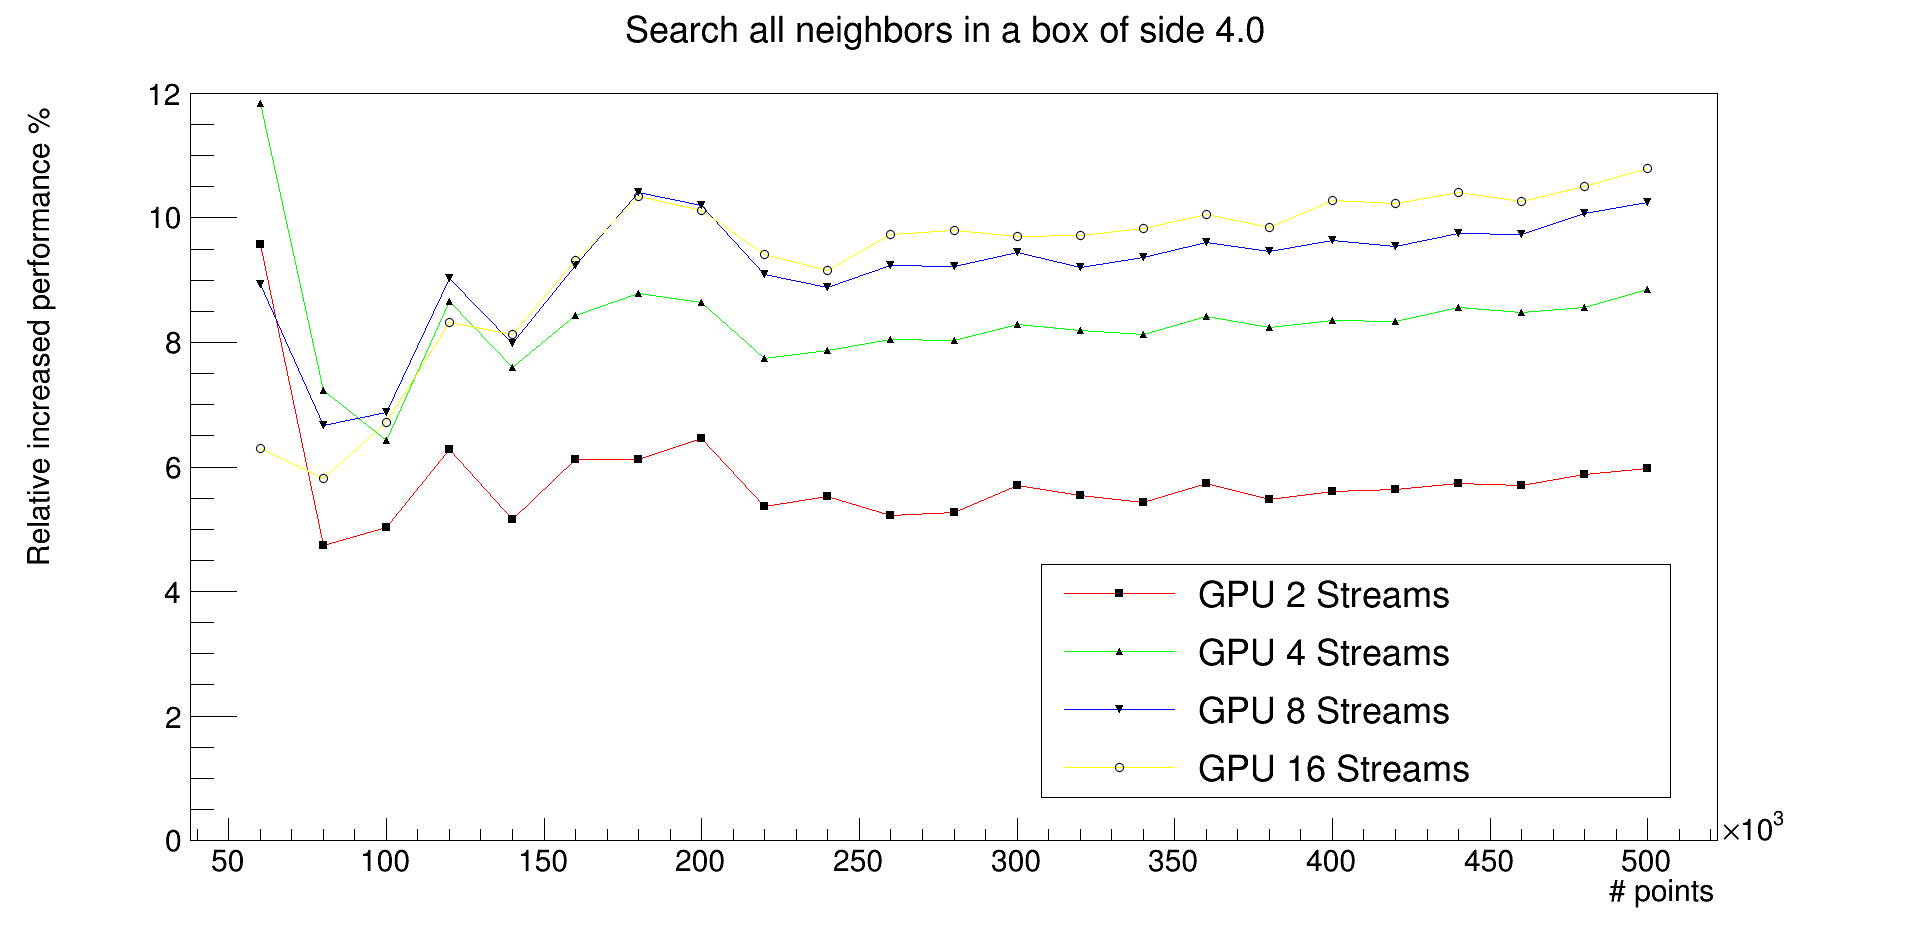
\includegraphics[width=\textwidth]{fkdtree/fkdStreams.png}
\caption{Relative performance gain between multiple CUDA streams with respect to the single stream.}
\label{fkdtree_streams}
\end{figure}

Following the results of the streams performance analysis we chose to use 8 CUDA streams to evaluate the performance of the GPU search with respect to the CPU one.\\

Figure \ref{fkdtree_search_times} shows the timings of the CPU sequential search and the GPU parallel one in the full range of the generated data sets, with the times shown in logarithmic scale.

\begin{figure}
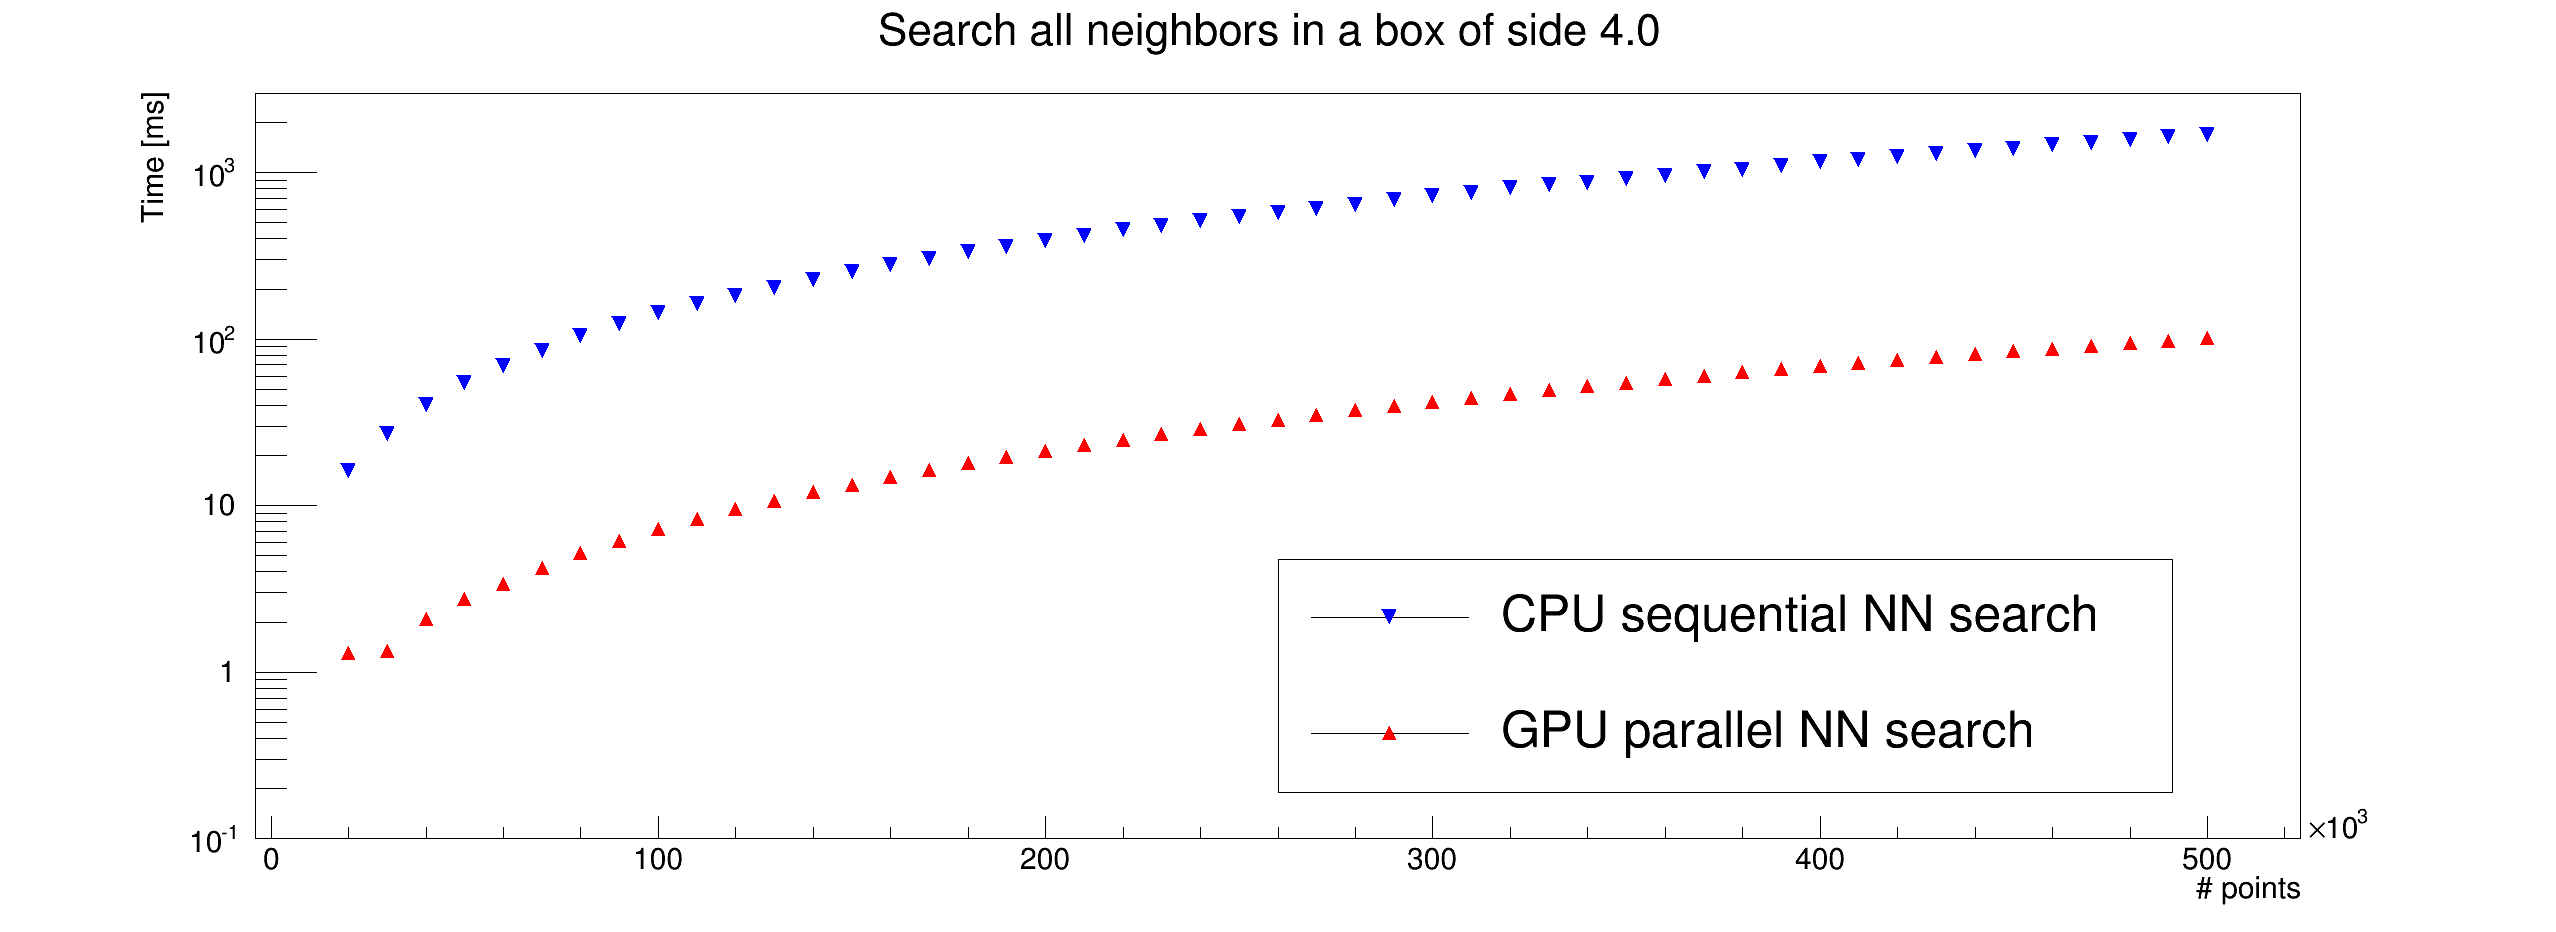
\includegraphics[width=\textwidth]{fkdtree/fkdSearchTimes.png}
\caption{Search times for CPU sequential and GPU parallel code.}
\label{fkdtree_search_times}
\end{figure}

Some selected timings are reported in Table \ref{fkdtree_times_tab}.\\

\begin{center}
\begin{table}[h]
\begin{tabular}{ c || r r r r r r r r r r }
Points ($10^{3}$) & 50 & 100 & 150 & 200 & 250 & 300 & 350 & 400 & 450 & 500 \\
\hline
CPU ($\unit{ms}$) & 54 & 142 & 253 & 384 & 539 & 714 & 907 & 1143 & 1384 & 1682 \\
GPU ($\unit{ms}$) & 3 & 7 & 13 & 21 & 31 & 42 & 54 & 68 & 84 & 101 \\
\end{tabular}
\caption{Selected search times for CPU sequential and GPU parallel code.}
\label{fkdtree_times_tab}
\end{table}
\end{center}

Lastly Figure \ref{fkdtree_speedup} shows the speedup between the two search methods.\\
\begin{figure}
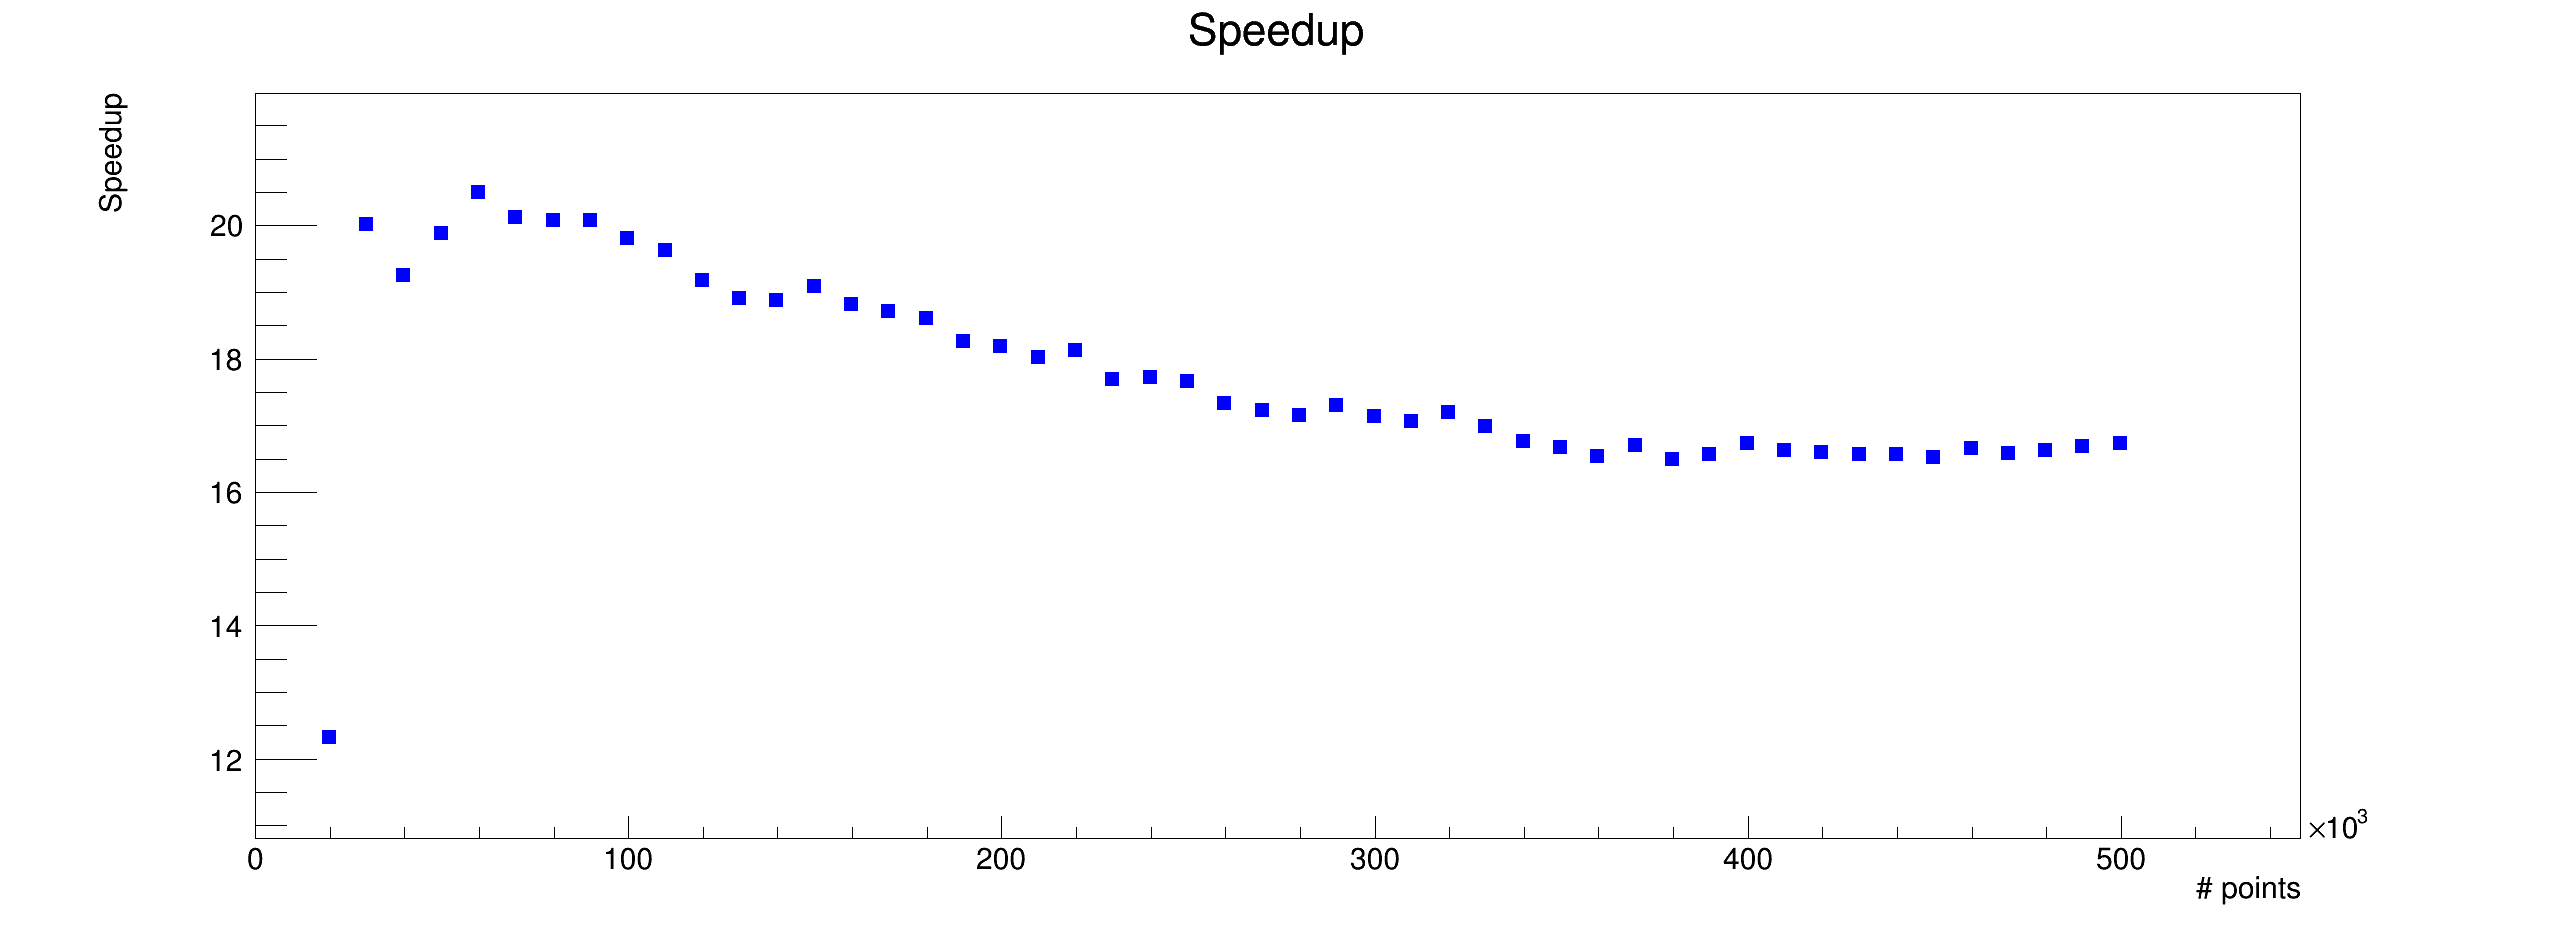
\includegraphics[width=\textwidth]{fkdtree/fkdSpeedup.png}
\caption{Speedup between CPU sequential and GPU parallel code.}
\label{fkdtree_speedup}
\end{figure}
\newpage

\subsection{HGCAL simulated RecHits}

We start off evaluating the algorithm performances on a simple -albeit not very realistic- simulation.
In several different events we instruct the simulation to generate a number of electrons of transverse momentum ($P_t$) between 10 $\unit{GeV/c}$ and 50 $\unit{GeV/c}$ starting from the central point of CMS and in a cone of pseudo-rapidity ($\eta$) comprised between 1.6 and 2.9 corresponding to the solid angle covered by HGCAL.\\
The generation of the electrons, the simulation of the detector response and the reconstruction of the \textit{rechits} -the points in HGCAL in which an energy deposit has been observed- are all handled by CMSSW: the CMS software package used by the collaboration to analyze and reconstruct the data from the experiment.\\
The points obtained are then passed to the KD-tree algorithm along with the search boxes to perform the all nearest neighbors search and evaluate the performance. The search boxes are defined by the Molière radius of a given layer of the detector. Thus when searching the nearest neighbors of a given rechit the layer of HGCAL it is situated on must be determined and so the Molière radius of that layer, as explained in Section \ref{sec:hgcal_clustering}.\\
We generate the events in set of: 4, 50, 120 and 200 electrons per event with the characteristics explained above. First we check the build times of the KD-tree to verify that is consistent with the behavior observed with the random points distribution, results are reported in Figure \ref{fkdtree_build_sim_times}.
Then we measure the search times for both CPU sequential and GPU parallel code, Table \ref{fkdtree_times_sim_tab} reports some selected results.
Figure \ref{fkdtree_search_times} shows all the times of the CPU and GPU searches on all the simulated data on a logarithmic scale.
Lastly Figure \ref{fkdtree_speedup} shows the speedup between the two searches.\\

\begin{figure}
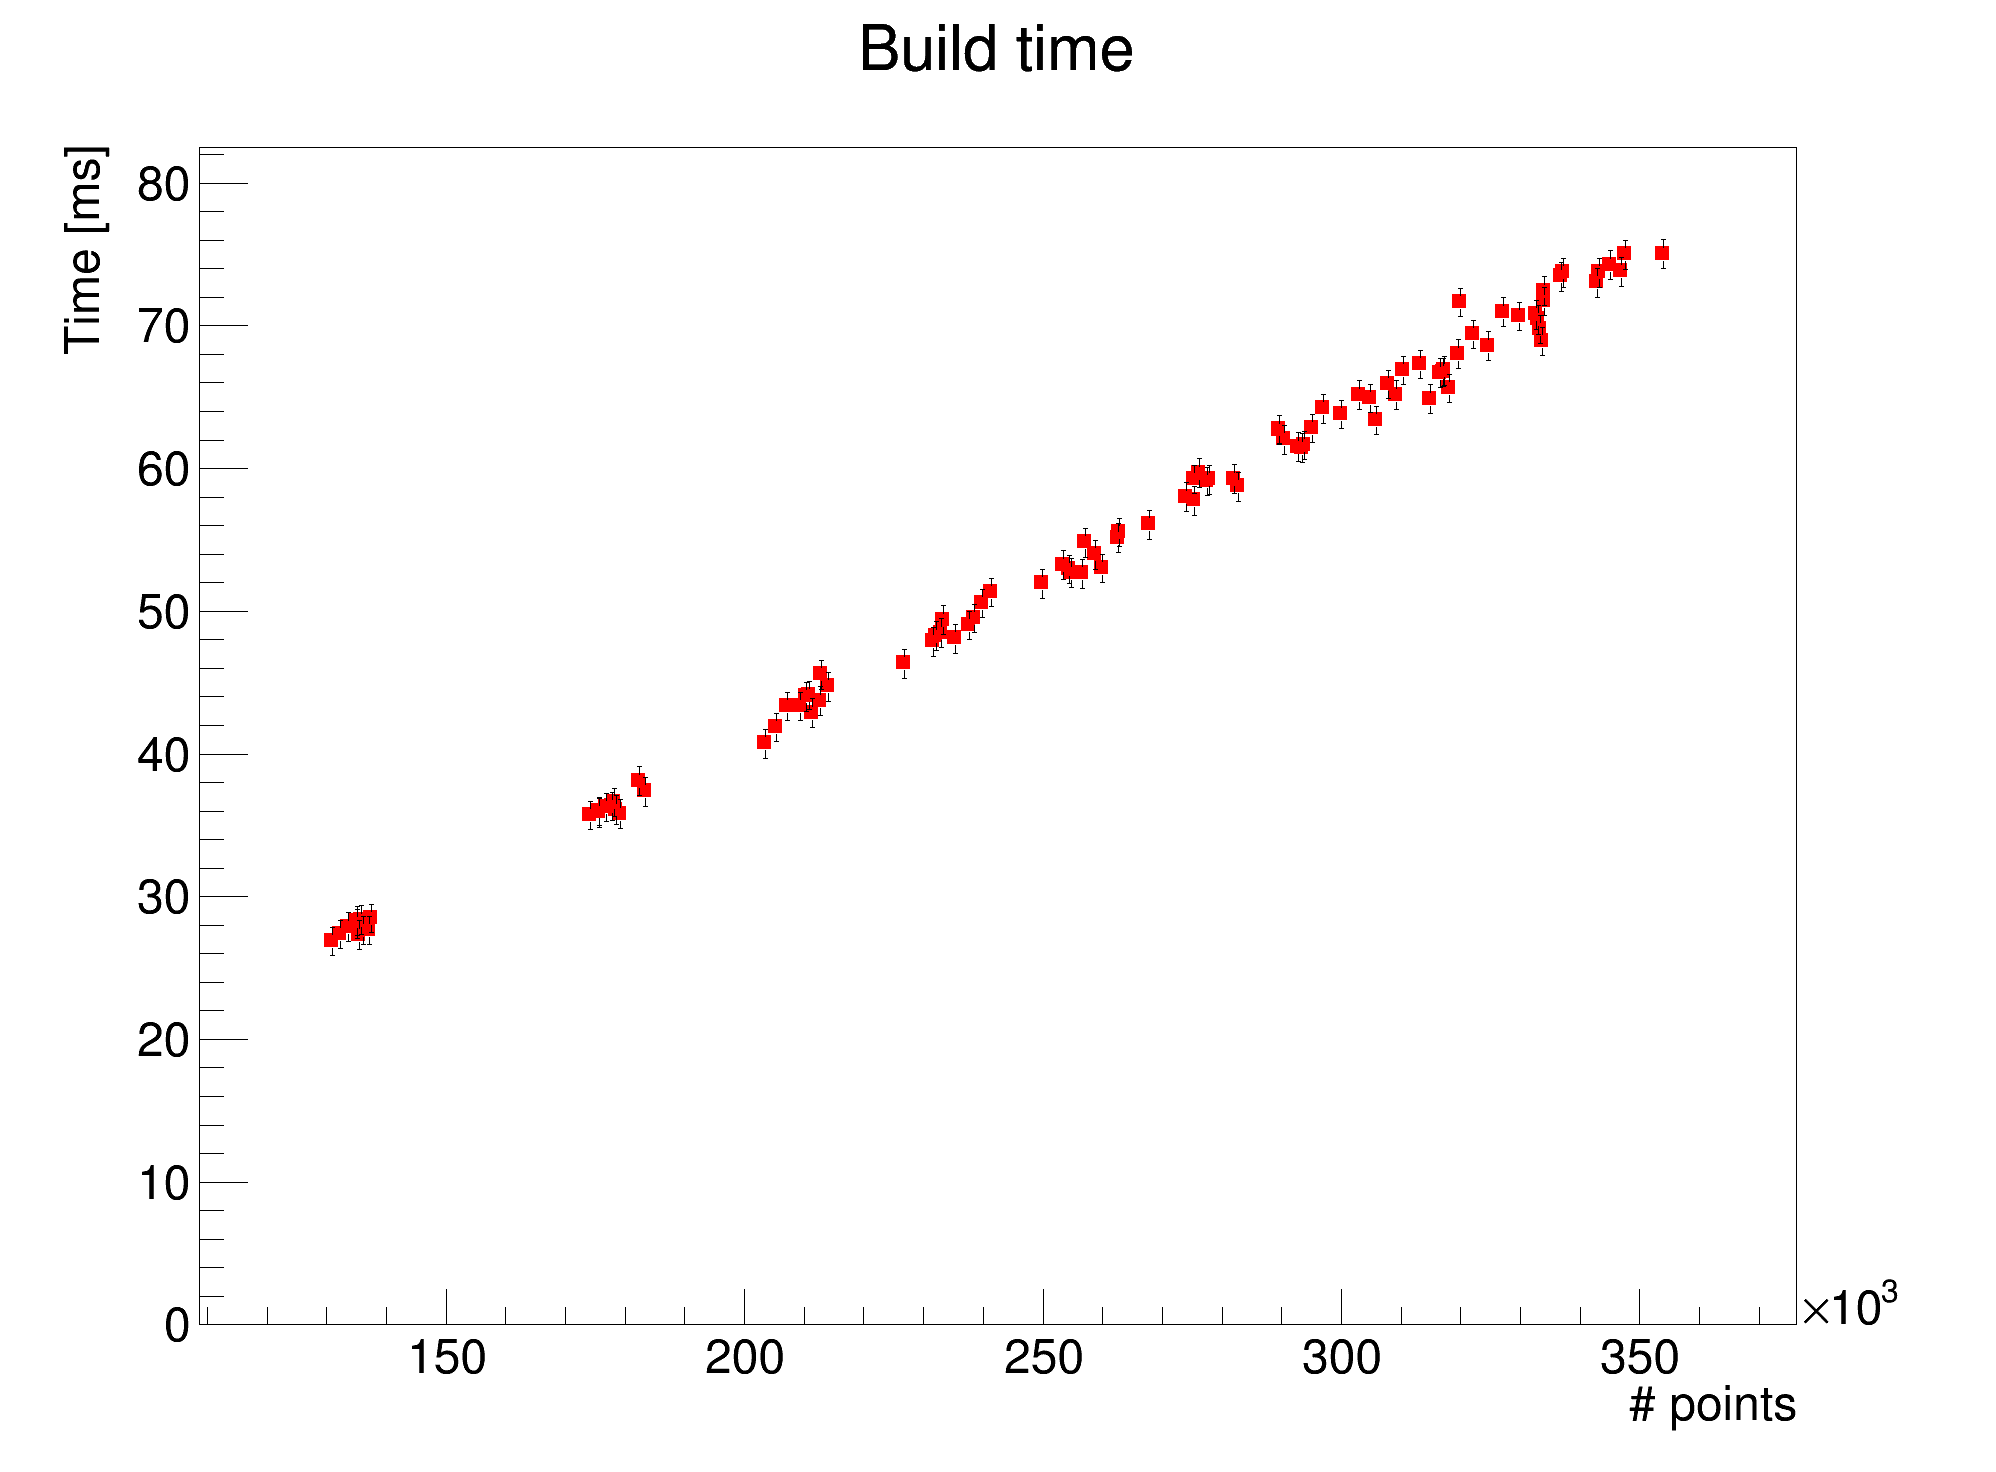
\includegraphics[width=\textwidth]{rechits/BuildTimes.png}
\caption{Time spent by the build of the KD-tree on simulated data.}
\label{fkdtree_build_sim_times}
\end{figure}

\begin{center}
\begin{table}[h]
\begin{tabular}{ c || r r r r r }
Points ($10^{3}$) & 37 & 139 & 225 & 260 & 362\\
CPU ($\unit{ms}$) & 21.59 & 144.8 & 320.4 & 266.9 & 518.7\\
GPU ($\unit{ms}$) & 3.388 & 10.69 & 19.17 & 22.87 & 34.54\\
\end{tabular}
\caption{Selected search times for CPU sequential and GPU parallel code searching simulated data.}
\label{fkdtree_times_sim_tab}
\end{table}
\end{center}

\begin{figure}
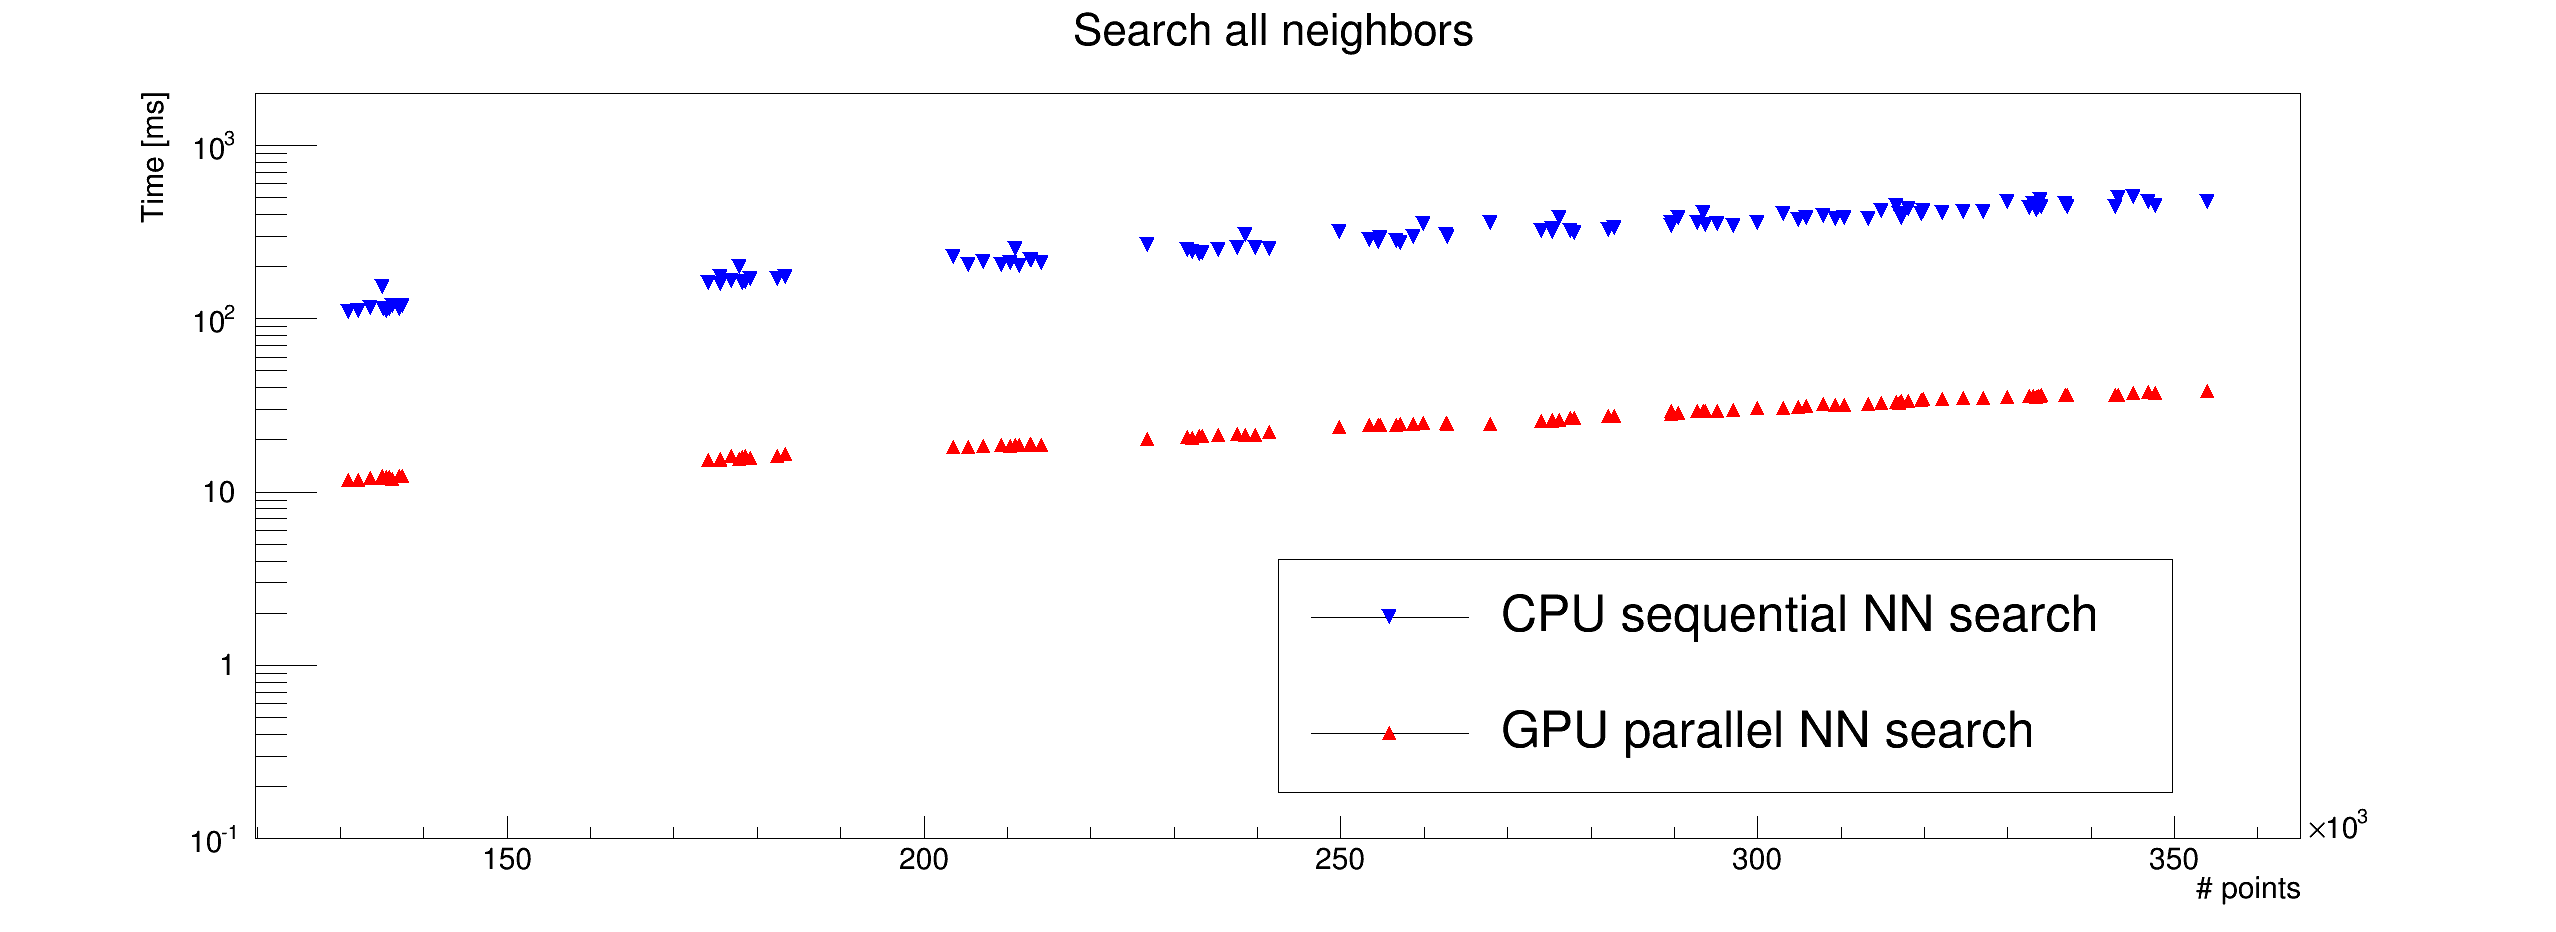
\includegraphics[width=\textwidth]{rechits/SearchTimes.png}
\caption{Search times for CPU sequential and GPU parallel code on simulated data.}
\label{fkdtree_search_times}
\end{figure}

\begin{figure}
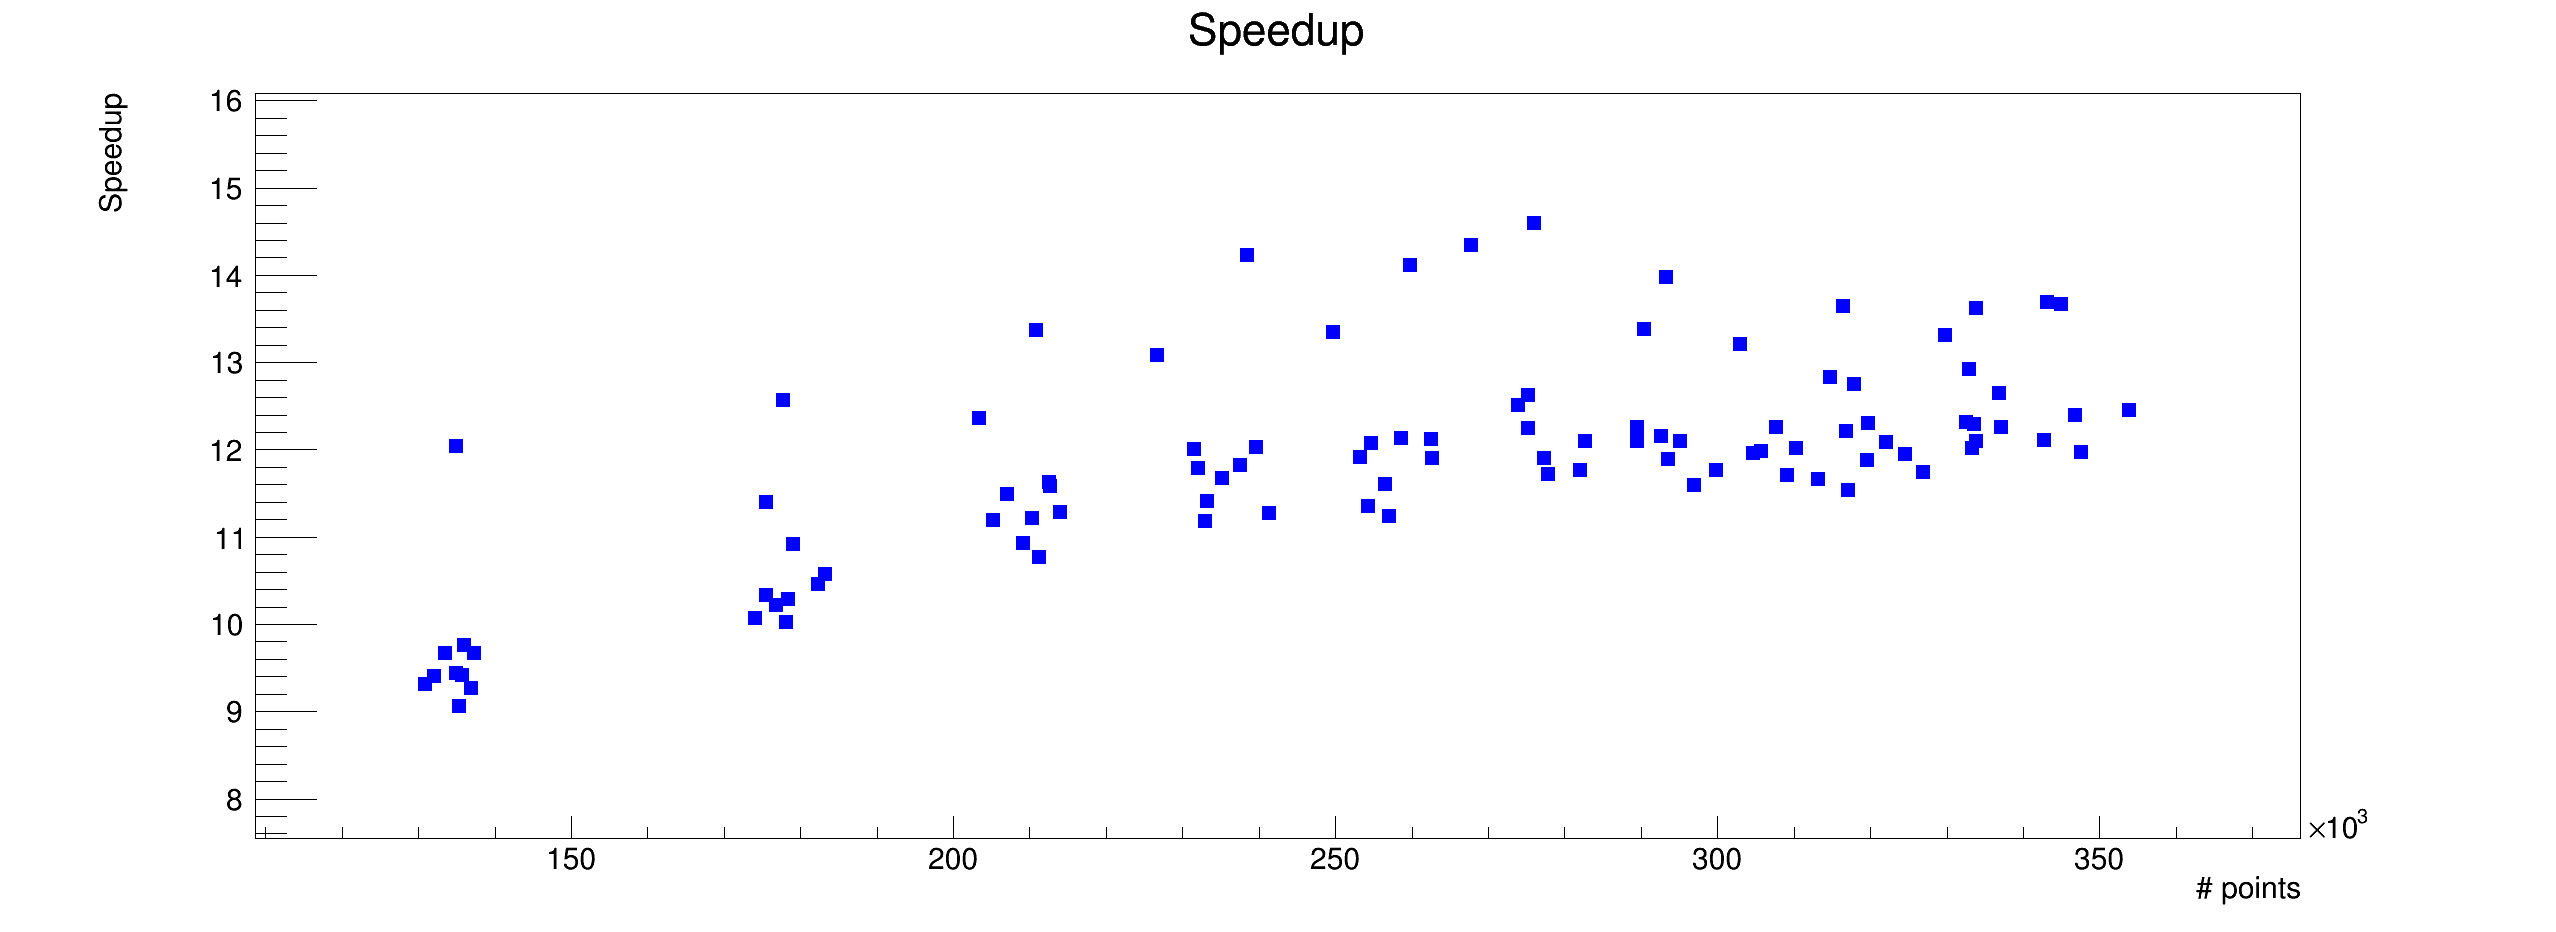
\includegraphics[width=\textwidth]{rechits/Speedup.png}
\caption{Speedup between CPU sequential and GPU parallel code on simulated data.}
\label{fkdtree_speedup}
\end{figure}
\\

\newpage

By observing the speedup plot we immediately realize there is some factor that can influence the speedup by up to $\sim 30\%$, indeed, while the timings of the GPU codes are compatibles with those obtained in the random generation case, the CPU code timings varies quite significantly. We attribute the variance to the random transverse momentum the electrons are generated with. Therefore it is necessary a further investigation of the algorithm performances with the variance of the $P_t$.


\subsubsection{Sets of constant $P_t$}

\section{Algorithm assessment}
\chapter{Power consumption}\label{ch:power}

\section{Benchmark machine}

\section{TK 1}

\section{TX 1}

\section{Consumption comparisons}
\chapter{Conclusions}\label{ch:conclusion}
The HL-LHC conditions of Phase-II will produce a great quantity of interactions in each event, rising the average pileup to 140 with spikes of 200. To ready the detector for Phase-II the CMS electromagnetic calorimeters endcaps will be upgraded with a new highly segmented sampling calorimeter: HGCAL. As we showed in Chapter \ref{ch:intro} for the above reasons it is expected that both the online and offline reconstructions will have to process a big number of \textit{rechits} in each event. Indeed, to reconstruct the electromagnetic clusters, it will be necessary to search for all the nearest neighbors of between 150000 and 350000 points, and for that reason the computational power required will need to increase substantially with respect to what it is available today.
\vspace{0.5cm}
\\
In Chapter \ref{ch:gpu} we described the most relevant differences between a Central Processing Unit and a Graphical Processing Unit. We showed how GPUs, that where made for a completely different purpose, can be leveraged to execute massively parallel programs thanks to the high number of cores they features. We described how a particular brand, NVIDIA, provides an extensive programming API for their GPU called CUDA and which features of CUDA can really benefit the parallel execution of a program.
\vspace{0.5cm}
\\
One of the most promising algorithms to perform the all nearest neighbors search is the binary K-Dimensional tree, in short KD-tree. In Chapter \ref{ch:volume_kd} we described the general properties of a KD-tree, how it is built and how it can be traversed to perform the nearest neighbors search. We also showed an implementation, which we refers to as Volume KD-tree since it uses three-dimensional volume as nodes of the tree, featuring a sequential search that runs on CPU and a parallel one for the GPU. After a thorough performance analysis we observed that the shortcomings of this implementation where outweighing the features meant to increase the performances and moved on to a different implementation.
\vspace{0.5cm}
\\
Abandoning the idea of tree nodes as volumes and converting the recursions into iterations we designed an entirely different KD-tree in Chapter \ref{ch:fkdtree}. The implementation proved to be much more suited to high parallelism and even more extensive performance testing where done. Beginning with random distributed points the algorithm showed very promising results in terms of both the absolute timing and the parallel code with respect to the sequential one. Another test using simulated data from the CMS software was executed and the good performance was still observed: the GPU code of the KD-tree is able to search the nearest neighbors of all 345000 simulated rechits in 37 $\unit{ms}$, with an effective speedup of almost 14 with respect to the sequential CPU code.
\vspace{0.5cm}
\\
We evaluated the energy consumption of the latter KD-tree on the workstation used throughout most of the work and also on the NVIDIA TK1 development board in Chapter \ref{ch:power}. First we compared the energy used by the workstation CPU (an Intel i7-3770) with the energy used by the GPU board mounted on the same machine (a NVIDIA Tesla k40c). We observed that, despite the power employment of the CPU is scarce, the overall energy consumed is significantly lower for the GPU with $13 \pm 1 \unit{J/search}$ respect to the $88 \pm 1 \unit{J/search}$ required by the CPU. Similar results where found when comparing the TK1 CPU (an ARM Cortex A15) and its integrated GPU (NVIDIA Kepler). While the ARM CPU results where really unimpressive, requiring $219 \pm 3 \unit{J/search}$, the GPU once again proved to be very efficient with $11 \pm 1 \unit{J/search}$. Therefore in the chapter we demonstrated how a well designed algorithm running on GPU not only can have great performance but can also significantly limit the energy required to perform a full nearest neighbors search. Of particular interest are the very compact System-on-a-Chip like the one featured in the TK1: with a very small form factor and a very low power usage those systems could be mounted in great quantities in small spaces without requiring complex heat dissipation systems, thus making them a very interesting candidate for a dedicated High Level Trigger farm for HGCAL.
\vspace{0.5cm}
\\
Although in the years to come before the Long Shutdown 3 the computational hardware will certainly improve and possibly in ways that are not entirely predictable, we strongly believe that the parallel programming paradigm will remains a stronghold of the High Performance Computing. We clearly showed throughout this work how an efficient parallel program might be not trivial to design. As a direct consequence of the Moore's law still proving to be true, the future will bring both CPUs and GPUs with even more cores and soon designing the software to be massively parallel will become essential.
\vspace{0.5cm}
\\
The full code developed for this work can be freely consulted and downloaded online \cite{github}.
\bibliographystyle{ieeetr}
\bibliography{BibTex}%{}

\listoftables
\listoffigures

\end{document}